% \begin{generalinstructions}
% Make sure the notation is consistent, Predefine $\bar{R},I $ for example. Also, look over and rewrite theorems so that they fit together with the notation. Ensure consistency in number of dimensions.
% \end{generalinstructions}


%%%%%%%%%%%%%%%%%%%%%%%%%%%%%%%%%%%%%%%%%%%%%%%%%%%%%%%%%%%%%%%%%%%%%%%%%%%%%%%%%%%%%%%%%%%%%%
%%%%%%%% Mathematical finance
%%%%%%%%%%%%%%%%%%%%%%%%%%%%%%%%%%%%%%%%%%%%%%%%%%%%%%%%%%%%%%%%%%%%%%%%%%%%%%%%%%%%%%%%%%%%%%
\subsection{Mathematical finance}\label{sec:MathematicalFinance}
%\todo{What is Mathematical finance}
In mathematical finance, one is typically interested in the returns of financial assets, over discrete time steps, rather than their price \citet[p.~2]{Danielsson2011}. Let $P_{t_i}$ denote the price at time increment $t_i$, where $t_i$ is usually in daily time increments, but can be any unit of time. 


\subsubsection{Returns}
This section will introduce different types of returns, simple and log, as well as their different properties. These properties are for example return aggregation over time, portfolio return calculations, generation of new prices, and the bounds for returns. The reason for introducing different types of returns is to show the connections between financial returns and statistical distributions that in turn connect to the theory of copulas. 

Firstly we should introduce what financial returns on assets are. The return of a financial asset is the relative price change over a given time interval, often expressed as a percentage \citet[p.~2]{Danielsson2011}. One type of return is simple returns, defined in \Cref{def:simpleReturns}.

\begin{definition}\label{def:simpleReturns}
    \textbf{Simple-Returns} \citet[p.~3]{Danielsson2011}
    A \emph{simple return} is the percentage change in price, over time period $t_i$, indicated by $R_{t_i}$:
    \begin{align*}
        R_{t_i} = \frac{P_{t_i}-P_{t_{i-1}}}{P_{t_{i-1}}}.
    \end{align*}
\end{definition}

To aggregate several simple (daily) returns over some time (week) to the return over the whole period (week), one has to construct several change factors that are multiplied together before subtracting one. This aggregation process is described in \citet[p.~3]{Danielsson2011}, where the aggregated return over $n$ periods can be calculated as
\begin{align*}
    R_{t_{i}}(n) = (1+R_{t_{i}})(1+R_{t_{i-1}})(1+R_{t_{i-2}})\dots (1+R_{t_{i-n+1}}) -1 = \frac{P_{t_{i}}}{P_{t_{i-n}}}-1.
\end{align*}

In many situations, it is necessary to calculate the return of an entire portfolio of assets from its underlying asset returns. For simple returns, this is simply done by calculating a weighted average of the individual asset returns. \citet[p.~3]{Danielsson2011} describes the calculation of the portfolio return $R_{t_i,\mathrm{port}}$ for a portfolio with $K$ different assets as 
\begin{align*}
    R_{t,\mathrm{port}} = \sum_{k=1}^K w_kR_{t,k}.
\end{align*}

Many times, it can be useful to simulate new stock prices by using randomly generated returns. For simple returns, new prices can be calculated as
\begin{align*}
    P_{t_{i}} = P_{t_{i-1}}(1+R_{t_{i}}).
\end{align*}

The space in which realizations of returns can be observed differs for different types of returns. In \Cref{ex:BoundsSimpleReturns} the range for simple returns is derived. 

\begin{example}\label{ex:BoundsSimpleReturns}
    To see the bounds for simple returns, we investigate what happens as the stock price moves to zero, corresponding to bankruptcy, and when the stock price moves to infinity. We denote the simple return when the price goes to zero and infinity by $R_t^-$ and $R_t^+$ respectively   
    \begin{align*}
        R_{t_i}^- = \lim_{P_{t_i} \to 0} \frac{P_{t_i}-P_{t_{i-1}}}{P_{t_{i-1}}} = \frac{0-P_{t_{i-1}}}{P_{t_{i-1}}} =  -1 \\
        R_{t_i}^+ =\lim_{P_{t_i} \to \infty} \frac{P_{t_i}-P_{t_{i-1}}}{P_{t_{i-1}}} = \frac{\infty-P_{t_{i-1}}}{P_{t_{i-1}}}=\infty.\\    
    \end{align*}
Hence, we conclude that $R_t \in (R_t^-,R_t^+) = [-1,\infty)$. 
\end{example}


Continuously compounded returns or so-called logarithmic returns are often used for financial modeling given their desirable properties. A desirable property is that the returns are \emph{symmetric}, so positive and negative returns of the same magnitude cancel each other out \citet[p.~4]{Danielsson2011}. Log returns are defined, as done by \citet[p.~3]{Danielsson2011}, in \Cref{def:logReturns}. 

\begin{definition}\label{def:logReturns}
    \textbf{Log-Returns} \\
    The logarithm of gross return or \emph{log-returns}, indicated by $Y_{t_i}$:
    \begin{align*}
        Y_{t_i} = \mathrm{log}(1+R_{t_i}) = \mathrm{log} \left(\frac{P_{t_i}}{P_{t_{i-1}}}\right) = \mathrm{log}(P_{t_{i}}) -\mathrm{log}(P_{t_{i-1}})
    \end{align*}
\end{definition}

Log-returns have the advantage that the multiperiod, $n$ period, returns are just the sum of one period returns \citet[p.~3]{Danielsson2011}, that is 
\begin{align*}
    Y_{t_i}(n) = Y_{t_i}+Y_{t_{i-1}} + \dots + Y_{t_{i-n+1}}.
\end{align*}

 
As illustrated by \citet[p.~4]{Danielsson2011}, the portfolio return is more complicated to compute for log returns because the relation is not simply a weighted sum
\begin{align*}
        Y_{t_i,\mathrm{port}} &= \mathrm{log}\left(\frac{P_{t_i,\mathrm{port}}}{P_{t_{i-1},\mathrm{port}}}\right) \neq  \sum_{k=1}^K w_k\mathrm{log}\left(\frac{P_{t_i,k}}{P_{t_{i-1},k}}\right), \mathrm{where} \;\\
        P_{t_i,\mathrm{port}} &= \sum_{k=1}^K w_k P_{t_i,k}.
\end{align*}


A weighted average is approximately, but not quite correctly, describing the portfolio returns in terms of the individual returns as described by \citet[p.~3]{Danielsson2011},
\begin{align*}
    Y_{t_i,\mathrm{port}} \approx \sum_{k=1}^K w_k R_{t_i,k}.
\end{align*}

The correct relation between portfolio log returns and its sub-components log returns is given by first converting the log returns to prices, then calculating the portfolio returns before calculating the log return from the portfolio return
\begin{align*}
    Y_{t_i,\mathrm{port}} = \mathrm{log} \left( \frac{\sum_{k=1}^K w_k P_{t_i,k}}{\sum_{k=1}^K w_k P_{t_{i-1},k}}\right), \mathrm{where} \; P_{t_i,k} = P_{t_i-1,k}e^{Y_{t_i,k}}.
\end{align*}
In the above expression, the nominator represents the new portfolio value while the denominator represents the initial portfolio value. $K\in \mathbb{N}$ is the number of assets in the portfolio and $w_k$ is the weight of the total portfolio in asset $k$. Note that the individual asset prices are updated, using the log return, by themselves before weighing them together as a portfolio value. 

In many applications, one wants to simulate returns to produce artificial stock price developments. Log returns from stock prices usually seem to be generated from some sort of bell-shaped probability distribution. This makes it convenient becausecause one can use samples from some probability distribution as the log returns when simulating prices for an asset. As an example, the famous Black-Scholes model assumes that stock returns are log normally distributed. That is, the log returns are normally distributed. 

%\todo{what to do with t here?}
To obtain the price $P_{t_i}$ at the end of time period $t_i$ using a simulated log return $Y_{t_i}$ for period $t_i$, one can calculate 
\begin{align*}
    P_{t_i} = P_{t_{i-1}}e^{Y_{t_i}}. %(own)
\end{align*}

The range in which log returns can be observed is, unlike those in the simple return case, unbounded both positively and negatively. 
\begin{example}
    To see this we investigate what happens to the returns when the stock price moves to zero, corresponding to bankruptcy, and when the stock price moves to infinity. We denote the log return when the price goes to zero and infinity by $Y_t^-$ and $Y_t^+$ respectively.   
    \begin{align*}
        Y_{t_i}^- = \lim_{P_{t_i} \to 0} \mathrm{log} \left( \frac{P_{t_i}}{P_{t_{i-1}}}\right) = \mathrm{log}(0)= -\infty\\
        Y_{t_i}^+ =\lim_{P_{t_i} \to \infty} \mathrm{log}\left( \frac{P_{t_i}}{P_{t_{i-1}}}\right) = \mathrm{log}(\infty)= \infty\\    
    \end{align*}
    Hence, we conclude that $Y_{t_i} \in (Y_{t_i}^-,Y_{t_i}^+) = (-\infty,\infty)$. 
\end{example}

To better understand how the different types of returns work, \Cref{ex:returnSymmetry} shows that simple returns are not symmetrical whereas log returns are. 
\begin{example}\label{ex:returnSymmetry}
    \textbf{Symmetry of returns} (own example, on the same lines as \citet[p.~4]{Danielsson2011} but not quite)
    Consider an example of a stock having initial price $P_0 = 100$, price after one day $P_1 = 200$, and price at day two $P_2 = 100$. Let's examine what these price changes do to simple and log returns respectively.
    
    \textbf{Simple returns}\\
    The return on the first day is
    \begin{align*}
        R_1 = \frac{P_1-P_0}{P_0} = \frac{200-100}{100} = 1 = 100\%.
    \end{align*}
    The return on the second day is
    \begin{align*}
        R_2 = \frac{P_2-P_1}{P_1} = \frac{100-200}{200} = -\frac{1}{2} = -50\%.
    \end{align*}    
    \textbf{Log returns}\\
    The return on the first day is 
    \begin{align*}
       Y_1 = \log \left( \frac{P_1}{P_0}\right) = \log\left(\frac{200}{100}\right)  = \log(2) \approx 69 \%.
    \end{align*}
    The return on the second day is
    \begin{align*}
        Y_2 = \log\left(\frac{P_2}{P_1}\right) = \log\left(\frac{100}{200}\right)= \log\left(\frac{1}{2}\right) \approx -69\%.
    \end{align*}
    We can see that the log returns are symmetrical so that monetary gains and losses of equal magnitude have log returns of equal magnitude. This is in contrast to simple returns where gains and losses are not symmetrical.
\end{example}



%%%%%%%%%%%%%%%%%%%%%%%%%%%%%%%%%%%%%%%%%%%%%%%%%%%%%%%%%%%%%%%%%%%%%%%%%%%%
%%%% GBM
%%%%%%%%%%%%%%%%%%%%%%%%%%%%%%%%%%%%%%%%%%%%%%%%%%%%%%%%%%%%%%%%%%%%%%%%%%%%
\subsubsection{Geometric Brownian motion}
The symmetrical property of log returns is desirable because it means that the log returns can be modeled using a normal distribution. This is a convenient because the normal distribution has many nice properties and is easy to work with. Log returns are often used in financial modeling, perhaps most notably in the Black-Scholes model, for option pricing, where stock prices are assumed to follow a \gls{GBM} which price is log normally distributed. This is a consequence of the log returns being normally distributed. The \gls{GBM} is a stochastic process that is used to model the evolution of stock prices. The \gls{GBM} is defined by the stochastic differential equation (SDE)
\begin{align*}
    dS_t &= \mu S_t dt + \sigma S_t dW_t \\
    S_0 &= s_0, 
\end{align*}
where $S_t$ is the stock price at time $t$, $\mu$ is the drift, $\sigma$ is the volatility, and $W_t$ is a Wiener process \Citet[p.~67]{Bjork2019Edition3} \todo{Version Of Book}. The \gls{GBM} can be solved using the Itô formula, which gives the solution
\begin{align*}
    S_t = s_0 \;\mathrm{exp}\left( \left( \mu - \frac{\sigma^2}{2} \right)t + \sigma W_t \right),
\end{align*}
\Citet[p.~69]{Bjork2019Edition3}.

%%%%%%%%%%%%%%%%%%%%%%%%%%%%%%%%%%%%%%%%%%%%%%%%%%%%%%%%%%%%%%%%%%%%%%%%%%%%
%%%% Euler Maruyama
%%%%%%%%%%%%%%%%%%%%%%%%%%%%%%%%%%%%%%%%%%%%%%%%%%%%%%%%%%%%%%%%%%%%%%%%%%%%
\subsubsection{Euler-Maruyama Scheme}
To approximately simulate \gls{SDE}s the Euler-Maruyama scheme can be used. The Euler-Maruyama scheme is a numerical method for solving \gls{SDE}s. 

For an \gls{SDE} of the form
\begin{align*}
    dX_t = a(X_t)dt + b(X_t)dW_t,
\end{align*}
the Euler-Maruyama scheme is defined as follows. 
Let $\hat{X}$ denote the approximate solution to the \gls{SDE} and let $X$ denote the exact solution. The Euler-Maruyama scheme is defined by the following recursive formula 
\begin{align*}
    \hat{X}(t_{i+1}) = \hat{X}(t_i) + a(\hat{X}(t_i))[t_{i+1}-t_i]  + b(\hat{X}(t_i)) \sqrt{t_{i+1}-t_i} Z_{i+1},
\end{align*}
where $Z_{i+1}$ is a standard normal random variable. The time step $t_{i+1}-t_i$ is the time increment, and $a$ and $b$ are the drift and diffusion functions respectively \Citet[pp.~339-340]{glasserman2004monte}.

We can use the Euler-Maruyama scheme to simulate a stock trajectory with the \gls{GBM} by setting $a(S_t) = \mu S_t$ and $b(S_t) = \sigma S_t$. The resulting scheme is
\begin{align*}
    \hat{S}(t_{i+1}) = \hat{S}(t_i) + \mu \hat{S}(t_i)[t_{i+1}-t_i]  + \sigma \hat{S}(t_i) \sqrt{t_{i+1}-t_i} Z_{i+1}.
\end{align*}
To simulate a stock trajectory, the time increment $t_{i+1}-t_i$ is set to a small value, and the process is iterated for a large number of steps. 

We can simulate a pair of dependent stock trajectroies by simulating a system of \gls{GBM}s  
\begin{align*}
    dS_t^d = \mu S_t^d dt + \sigma S_t^d dW_t^d, \; d=1,2, 
\end{align*}
where $W_t^1$ and $W_t^2$ are standard one dimensional Wiener processes with correlation $\rho$ \Citet[p.~104]{glasserman2004monte}. One can also simulate a system of \gls{GBM}s with a dependence different than correlation. This can be done by using a copula to generate the dependent Weiner processes. \todo{Need reference for this?}


In financial applications one is often interested in what impact changes in asset prices have on the value of a financial instrument and risk metrics. To do this a widely used method is to simulate the future price of the underlying asset and then calculate how the value of the instrument or metric changes based on the simulated prices. This allows for the calculation of risk metrics such as \gls{VaR} and \gls{ES} as well as the pricing of financial instruments such as options. The method is often referred to as Monte Carlo simulation.  

%%%%%%%%%%%%%%%%%%%%%%%%%%%%%%%%%%%%%%%%%%%%%%%%%%%%%%%%%%%%%%%%%%%%%%%%%%%%
%%%% Monte Carlo methods
%%%%%%%%%%%%%%%%%%%%%%%%%%%%%%%%%%%%%%%%%%%%%%%%%%%%%%%%%%%%%%%%%%%%%%%%%%%%
\subsubsection{Monte Carlo methods} \label{sec:MonteCarlo}
\begin{generalinstructions}
    \textbf{I would say}\\
    Monte Carlo methods is a blanket term for computational methods that utilize random numbers to model uncertain events. Given an assumption about the underlying distribution of a random process. The random process is simulated multiple times and used as the input in a deterministic function, the result of which is averaged. 
\end{generalinstructions}

Many times in different scientific fields, relationships between different variables can be described using deterministic relationships between input variables and output variables. In some situations, these deterministic relationships have random input parameters. In these cases, Monte Carlo methods can be useful. 

Monte Carlo simulation is a method for simulating events that, due to some source of randomness, are uncertain. In Monte Carlo methods, a statistical distribution is identified for each source of randomness. The method is then to sample random numbers from these distributions to use as input in the deterministic relationship. This gives the outcome for multiple possible scenarios. The final step is to perform some statistical analysis of the generated output values from the functions. This can, for example, be used to calculate the mean, standard deviation, or percentile \Citet[pp.~91-92]{Raychaudhuri2008}.
\todo{Connect to Mathematical finance}

%%%%%%%%%%%%%%%%%%%%%%%%%%%%%%%%%%%%%%%%%%%%%%%%%%%%%%%%%%%%%%%%%%%%%%%%%%%%%%%%%%%%%%%%%%%%%%
%%%%%%%% Probability theory
%%%%%%%%%%%%%%%%%%%%%%%%%%%%%%%%%%%%%%%%%%%%%%%%%%%%%%%%%%%%%%%%%%%%%%%%%%%%%%%%%%%%%%%%%%%%%%

\subsection{Probability theory}
As mentioned above, stock returns are often modeled using some statistical distribution. Statistical distributions are fundamental to the theory of copulas and therefore we need to define the terminology around distributions more formally. Throughout the upcoming sections, illustrations will be made to explain the ideas visually. Unless otherwise stated the Gaussian distribution, with mean 0 and standard deviation 1, will be used for these illustrations.

First, we need to define what statistical distributions are, beginning with \gls{CDF} in one dimension defined in \Cref{def:CDF1d}.

\todo{Maybe write in terms of random variable?}

\begin{definition}\label{def:CDF1d} \textbf{CDF one dimension }  \citet[p.~17]{Nelsen2006}\\
    A \emph{distribution function} or \gls{CDF} is a function $F$ with domain $\bar{R} = [-\infty, \infty]$ such that 
    \begin{compactenum}
        \item $F$ is nondecreasing; 
        \item $F(-\infty)=0$ and $F(\infty)=1$.
    \end{compactenum}
\end{definition}

One can think of the \gls{CDF} at each point on its domain $\bar{R}$ as the probability of a realization being below that point. Tied to the \gls{CDF} is the \gls{PDF}, which is defined in \cref{def:PDF1d}.

\begin{definition}\label{def:PDF1d} \textbf{PDF one dimension} \citet[pp.~160-161]{DevoreBerk2012}\\
    Let $X$ be a continuous random variable. Then a \emph{probability distribution} or \gls{PDF} of $X$ is a function $f(x)$ such that for any two numbers $a$ and $b$ with $a \leq  b$,
        \begin{align*}
            P(a \leq X \leq b) = \int_a^bf(x)dx.\\
        \end{align*}
\end{definition}

\begin{remark}\label{rem:pdfProperties}
    Note that for a function to be a valid \gls{PDF}, the following conditions must be satisfied. 
    \begin{align*}
        f(x) \geq 0 \; \mathrm{ for\; all \;} x;\\
        \int_{-\infty}^{\infty}f(x)dx = 1. 
    \end{align*}
    These are implied by \Cref{def:PDF1d} but are explicitly stated here for clarity. 
\end{remark}


\Cref{fig:PDFandCDF1D} illustrates both a \gls{PDF} (left) and \gls{CDF} (right) for a random variable $X$, being standard normally distributed. In the left figure, we can see a histogram of simulated data generated from the standard normal distribution as well as the theoretical normal distribution. The \gls{PDF} shows the likelihood of a realization of the $X$ to end up at each point in the domain of $X$. The right picture shows the \gls{CDF} corresponding to the \gls{PDF}, its function value in each point is defined as the probability of ending up below that point on the domain of $X$.

\begin{figure}
    \centering
    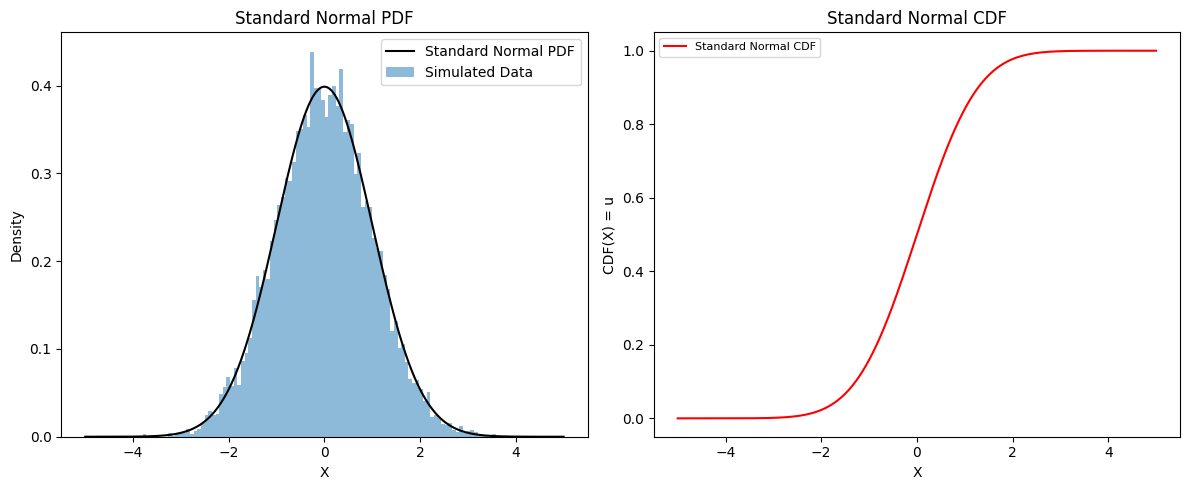
\includegraphics[width=1\linewidth]{3Theory/pictures/CDFandPDF1D.png}
    \caption{Illustration of a \gls{PDF} (left) and \gls{CDF} (right) for a random variable $X$, being standard normally distributed, in one dimension.}
    \label{fig:PDFandCDF1D}
\end{figure}

When dealing with multiple assets the notion of a \gls{CDF} generalizes to a multivariate \gls{CDF}. To define a multivariate \gls{CDF} formally in two dimensions we will need to define the $H$-volume of a function in two dimensions and what the meaning of a function being 2-increasing is. This is done in the same manner as in \citet[p.~8]{Nelsen2006} in \Cref{def:H-volume} and \Cref{def:2-Increasing}.

\begin{definition}\label{def:H-volume} \textbf{H-Volume} \citet[p.~8]{Nelsen2006}\\
    Let $u$ and $v$ be nonempty subsets of $\bar{R} = [-\infty, \infty]$, and let $H$ be a two-place real function such that $\D H = u\times v$. Let $B = [u_1,u_2]\times[v_1,v_2]$  be a rectangle all of whose vertices are in $\D H$. Then
    the \emph{H-volume} of $B$ is given by
    \begin{align*}
        V_H(B) = H(u_2,v_2) - H(u_2,v_1) - H(u_1,v_2) + H(u_1,v_1).
    \end{align*}
\end{definition}

\begin{definition}\label{def:2-Increasing} \textbf{2-increasing} \citet[p.~8]{Nelsen2006}\\
     A 2-place real function $H$ is \emph{2-increasing} if its $H$-volume $V_H(B)\geq0$, for all rectangles B whose vertices lie in $\D H$.
\end{definition}

The notion of a 2-increasing function is illustrated in \Cref{fig:2-Increasing}. In the figure, the left picture shows a function that is 2-increasing meaning that it is increasing in both directions. The right picture illustrates when a function is not 2-increasing and how this will be captured by the $H$-volume of the function. This property is needed to define a \gls{CDF} in several dimensions, as done by \citet[p.~17]{Nelsen2006}, in \Cref{def:JointCDF}. 

\begin{figure}
    \centering
    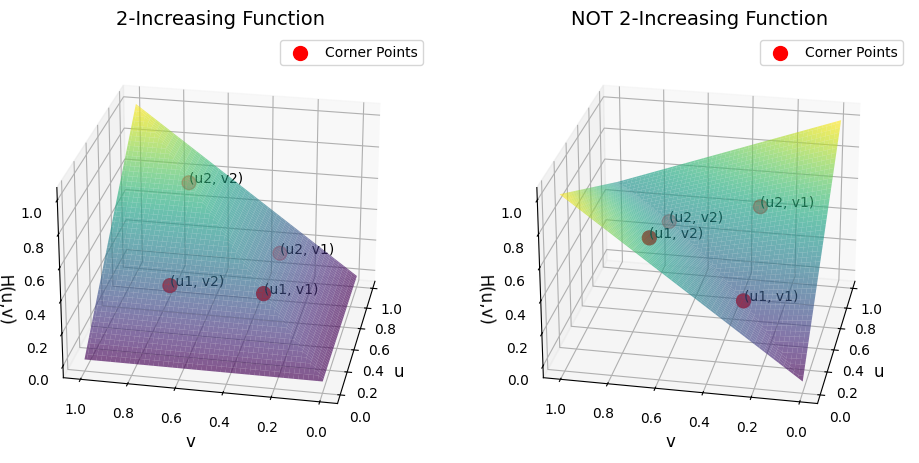
\includegraphics[width=1\linewidth]{3Theory/pictures/2increasingAndNot.png}
    \caption{Illustration of what it means for a function to be, and not to be, 2-increasing using the definition of the $H$-volume.}
    \label{fig:2-Increasing}
\end{figure}
%\todo{Maybe rotate?}


\begin{definition}\label{def:JointCDF} \textbf{Joint CDF} \\
    A \emph{joint distribution function} or joint \gls{CDF} is a function $F$ with domain $\bar{R}^2 = [-\infty, \infty]^2$ such that 
    \begin{compactenum}
        \item $F$ is 2-increasing; 
        \item $F(x_1,-\infty)= F(-\infty, x_2) = 0$, and $F(\infty,\infty)=1$.
    \end{compactenum}
\end{definition}

As in the univariate case the function value of the joint \gls{CDF} at any point in $\mathrm{Dom}X\times\mathrm{Dom}Y$ $\bar{R}^2$ is the probability of being below that point. In the two-dimensional setting, it is the probability of a point ending up below the point in both dimensions simultaneously. 

We can also define a \gls{PDF} in two dimensions as done by \citet[p.~235]{DevoreBerk2012} in \Cref{def:JointPDF}.

\begin{definition}\label{def:JointPDF} \textbf{Joint PDF} \\
    Let $X$ and $Y$ be continuous random variables. Then $f(x, y)$ is the \emph{joint} \gls{PDF} for $X$ and $Y$ if for any two-dimensional set $A$ 
    \begin{align*}
        P[(X,Y) \in A] =  \iint_A f(x,y)dxdy.
    \end{align*}
    
    In particular, if $A$ is the two-dimensional rectangle $\{(x,y) : a\leq x \leq b, c\leq y \ \leq d\}, $ then
    \begin{align*}
        P[(X,Y) \in A] = P(a\leq X \leq b, c \leq Y \leq d) =\int_a^b\!\!\!\int_c^d f(x,y)dxdy.
    \end{align*}
\end{definition}

\begin{remark}
    As seen in the univariate case, the same applies to the bivariate case. To be a candidate to be a joint \gls{PDF} $f(x,y)$ must satisfy 
    \begin{align*}
        &f(x,y) \geq 0, \;\mathrm{and} \\
        &\int_{-\infty}^{\infty}\!\int_{-\infty}^{\infty}f(x,y)dxdy=1.
    \end{align*}    
\end{remark}


Analogously to the univariate setting, the joint \gls{PDF} and \gls{CDF} are illustrated to give a visual understanding. In \Cref{fig:JointCDFandPDF} the left picture shows a joint \gls{PDF} for the random variable $X = (X_1, X_2)$, being standard normally distributed with zero correlation. In the right picture, the joint \gls{CDF} is displayed. 

\begin{figure}
    \centering
    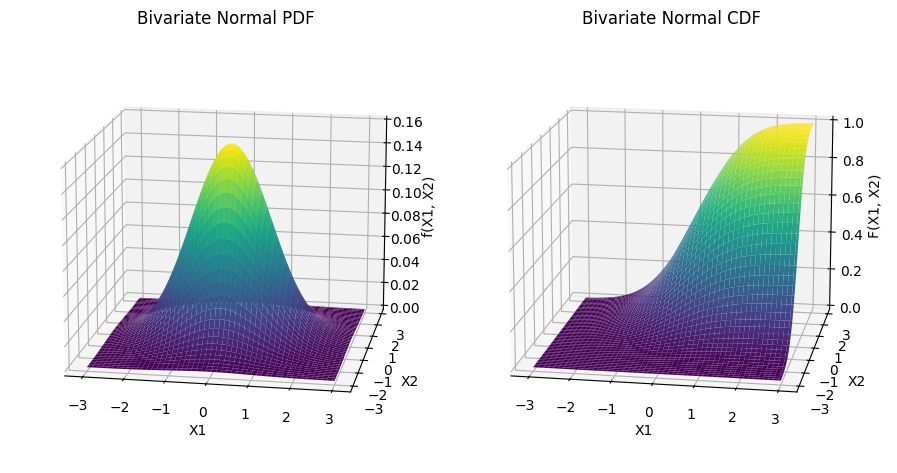
\includegraphics[width=1\linewidth]{3Theory/pictures/MultivariatePDFandCDF.png}
    \caption{Illustration of a \gls{PDF} (left) and \gls{CDF} (right) for a two dimensional random variable $X = (X_1,X_2)$, being standard normally distributed.}
    \label{fig:JointCDFandPDF}
\end{figure}


The \gls{PIT} refers to transforming a continuous random variable to a uniformly distributed random variable. 
This maps the domain of a continuous one-dimensional random variable through its \gls{CDF} to the $[0,1]$ space, which may in the sequel be referred to as \emph{probability space}. This transformation will be central when defining copulas and is introduced in \Cref{the:PIT} as done in \citet[p.~27]{Danielsson2011}. 

\begin{theorem}\label{the:PIT} \textbf{Probability integral transform} \\
    Let $X$ be a continuous random variable with distribution function $F$. Define a new random variable $U = F(X)$, then $U \sim \mathrm{unif}(0,1)$. 
\end{theorem}

The probability integral transform is illustrated in \Cref{fig:PIT}. We can think of the \gls{PIT} as a method of mapping all observed data points on $\D X$  to probability space. In the figure, this can be seen as the dotted lines representing data points being mapped. 




Deeply connected to the \gls{PIT} is the inverse transform method, which is a method of generating random numbers from a given distribution. The method is based on the \gls{PIT} and works as defined by \Citet[p.~54]{glasserman2004monte}.
\begin{definition}\label{def:InverseTransformMethod}
    \textbf{Inverse transform method} \\
    The \emph{inverse transform method} is a method of generating random numbers from a given distribution.
    \begin{compactenum}
        \item Generate random numbers $U \sim \mathrm{Unif}(0,1)$;
        \item Insert the random numbers in the inverse \gls{CDF} of the desired distribution such that $X = F^{-1}(U)$.
    \end{compactenum}
    The random variable $X$ will then be distributed according to the desired distribution. That is $P(X\leq x) = F(x)$ for all $x$.
\end{definition}

The inverse transform method is illustrated in \Cref{fig:ITM} and can be seen as performing the \gls{PIT} in reverse. In the figure the red line is the inverse \gls{CDF} from which the sample is desired to be. The dotted lines represent the random numbers generated from the uniform distribution. The random numbers are then inserted into the inverse \gls{CDF} to obtain the desired sample.

\begin{figure}[h]
    \centering
    \begin{subfigure}[t]{0.45\linewidth}
        \centering
        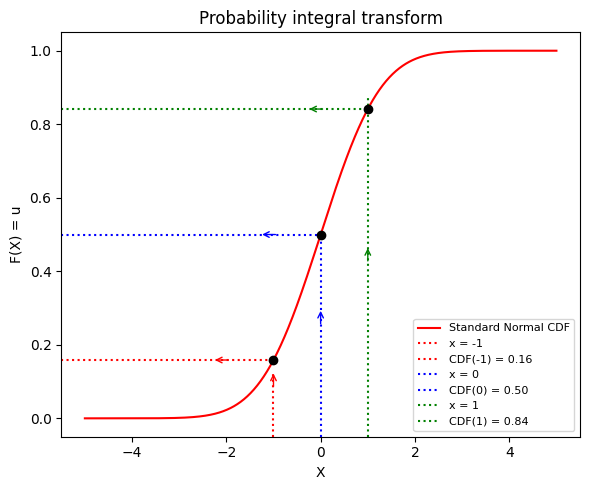
\includegraphics[width=\linewidth]{3Theory/pictures/ProbabilityIntegralTransform.png}
        \caption{Illustration of how the probability integral transform is used to transform realizations of a random variable $X$ having distribution function $F$ into a uniformly distributed random variable $U = F(X)$.}
        \label{fig:PIT}
    \end{subfigure}
    \hfill
    \begin{subfigure}[t]{0.45\linewidth}
        \centering
        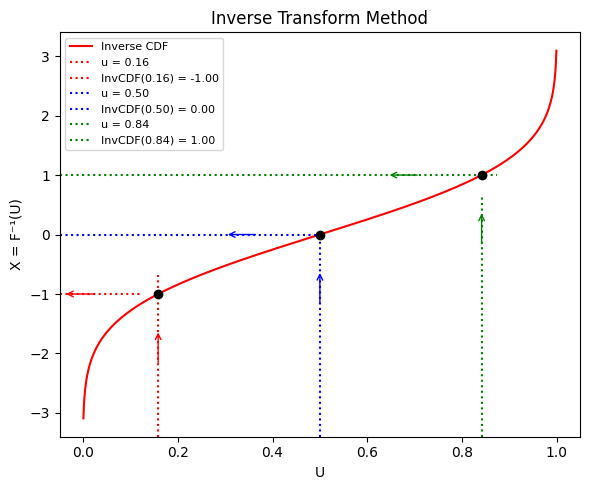
\includegraphics[width=\linewidth]{3Theory/pictures/InverseTransformMethod.png}
        \caption{Illustration of the inverse transform method and how it is used to generate random numbers from a given distribution given sampled points from a uniform distribution.}
        \label{fig:ITM}
    \end{subfigure}
    \caption{Probability Integral Transform and Inverse Transform Method.}
    \label{fig:TransformMethods}
\end{figure}


% \begin{figure}
%     \centering
%     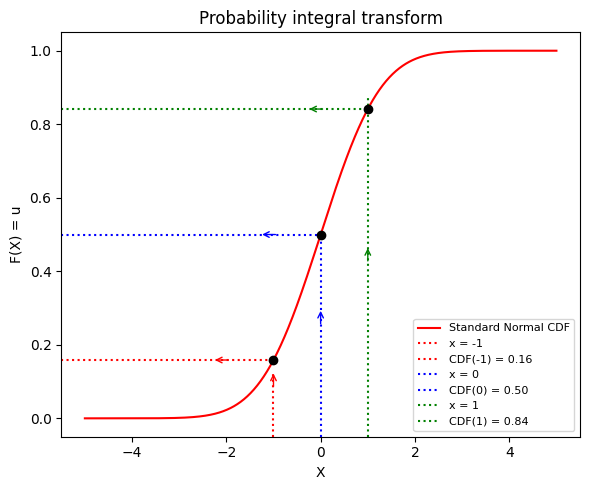
\includegraphics[width=0.45\linewidth]{3Theory/pictures/ProbabilityIntegralTransform.png}
%     \caption{Illustration of how the probability integral transform is used to transform realizations of a random variable $X$ having distribution function $F$ into a uniformly distributed random variable $U = F(X)$. }
%     \label{fig:PIT}
% \end{figure}
% \begin{figure}
%     \centering
%     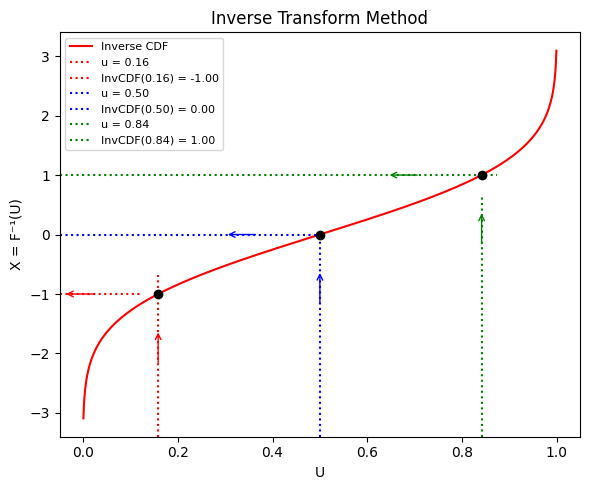
\includegraphics[width=0.45\linewidth]{3Theory/pictures/InverseTransformMethod.png}
%     \caption{Illustration of the inverse transform method and how it is used to generate random numbers from a given distribution given sampled points from a uniform distribution.}
%     \label{fig:ITM}
% \end{figure}


Another important notion is that of a marginal distribution of a joint distribution, which can be thought of as the distribution if only considering one of the dimensions that the joint distribution is made up of. The marginal \gls{CDF} and \gls{PDF} are defined in \Cref{def:MarginalCDF} and \Cref{def:MarginalPDF} respectively, in the same way as in \citet[p.~81]{evans2004probability} and \citet[p.~34]{wasserman2010statistics} respectively. 

\begin{definition}\label{def:MarginalCDF}
    \textbf{Marginal \gls{CDF}} 
    Let $X$and $Y$ be two random variables having joint \gls{CDF} $F_{X,Y}$, then the \gls{CDF} $F_X$ of $X$ can be obtained from $F_{X,Y}$ because
    \begin{align*}
        F_X(x) =P(X\leq x)
        =P(X\leq x,Y \leq \infty)
        =\lim_{y\to\infty} F_{X,Y}(x,y).
    \end{align*}
    $F_X$ is called the \emph{marginal distribution function} or marginal \gls{CDF} of $X$. The marginal distribution $F_Y$ can be obtained similarly. 
\end{definition}

\begin{definition}\label{def:MarginalPDF}
    \textbf{Marginal \gls{PDF}}
    For a continuous random variable, with domain $\mathrm{Dom}X\times \mathrm{Dom}Y$ $f_{X,Y}$, having joint \gls{PDF} $f_{X,Y}$, the \emph{marginal density function} or marginal \gls{PDF} of $X$ is given by
    \begin{align*}
        f_X(x) = \int_{-\infty}^\infty f_{X,Y}(x,y)dy.
    \end{align*}
    The marginal density $f_Y$ can be obtained similarly. 
\end{definition}

In \Cref{fig:MarginalCDF} the notion of a marginal distribution is visualized. In the left figure, a joint \gls{CDF} is shown to connect to the prior explanation of a \gls{CDF}. If the distribution is rotated to show it straight from one direction, as shown in the right figure, we can see the marginal distribution. In this case, it is the marginal distribution of $X_2$ that is displayed in red. This figure is of course simplified as it would not be plausible to view the limit when $X_1 \to \infty$.

\begin{figure}
    \centering
    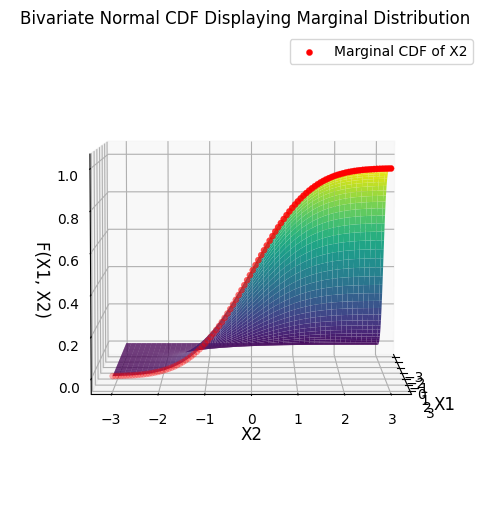
\includegraphics[width=1\linewidth]{3Theory/pictures/MarginalIllustrated.png}
    \caption{Illustration of what the marginal \gls{CDF} looks like for a bivariate normal distribution.   }
    \label{fig:MarginalCDF}
\end{figure}

To conclude this subsection, we will show how the \gls{PIT} is utilized to transform data to the probability space and explain how it sets the stage for copulas. \Cref{fig:PITonData} illustrates how the \gls{PIT} is used to transform two-dimensional data into the two-dimensional probability space, by transforming through each of the marginal distributions separately. This is done for standard normally distributed data with and without correlation in (b) and (a) respectively, to highlight the differences in the distribution of points in the probability space when dependence is present and not in (d) and (c) respectively.

\begin{figure}
    \label{fig:PITonData}
    \centering
    \begin{minipage}{0.4\textwidth}
        \centering
        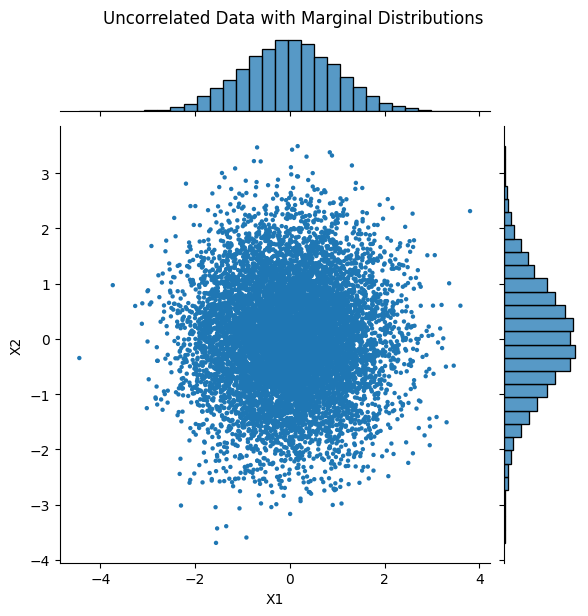
\includegraphics[width=\textwidth]{3Theory/pictures/UncorrelatedScatter.png}
        \subcaption{}
    \end{minipage}
    \hfill
    \begin{minipage}{0.4\textwidth}
        \centering
        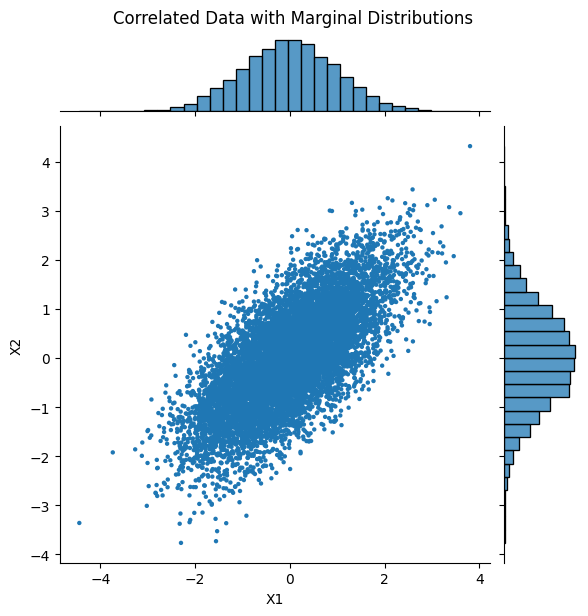
\includegraphics[width=\textwidth]{3Theory/pictures/CorrelatedScatter.png}
        \subcaption{}
    \end{minipage}
    \vfill
    \begin{minipage}{0.4\textwidth}
        \centering
        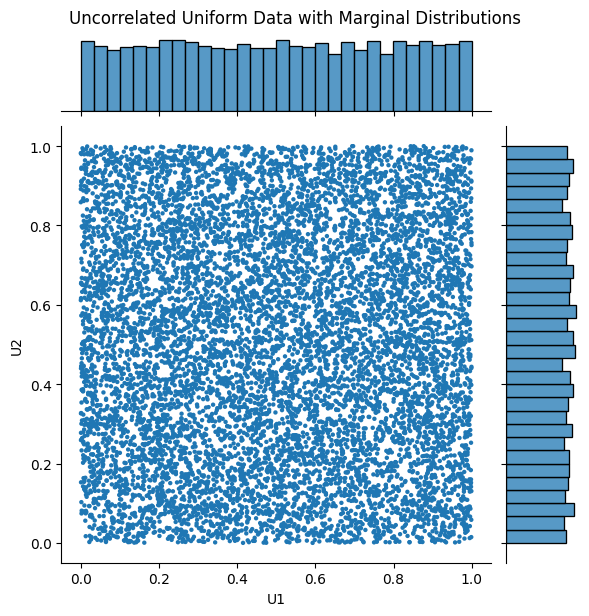
\includegraphics[width=\textwidth]{3Theory/pictures/UncorrelatedUniformScatter.png}
        \subcaption{}
    \end{minipage}
    \hfill
    \begin{minipage}{0.4\textwidth}
        \centering
        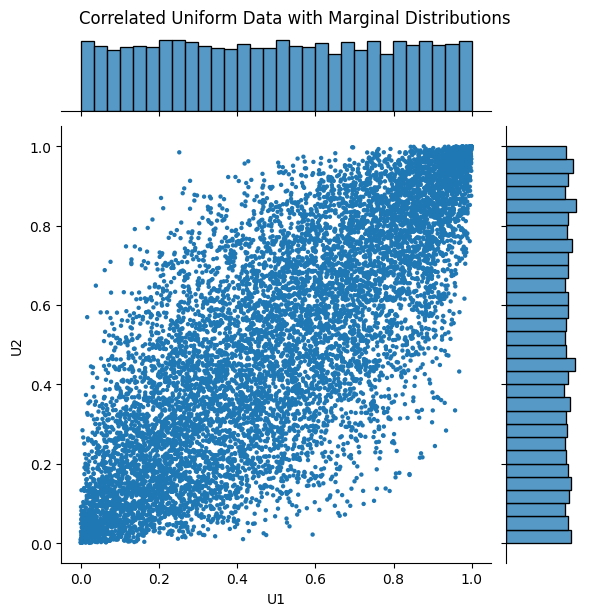
\includegraphics[width=\textwidth]{3Theory/pictures/CorrelatedUnoformScatter.png}
        \subcaption{}
    \end{minipage}
    \caption{Illustration of how the \gls{PIT} is used to transform two-dimensional data into the $[0,1]$-domain by considering the marginal distribution of each dimension separately.}
\end{figure}

Before introducing copulas in the next section we can simply describe the setting for copulas as \gls{CDF} of the data after having transformed it into the probability space using the \gls{PIT}. Relating to \Cref{fig:PITonData} we the copula is the \gls{CDF} of the data in (c) or (d).


\textbf{Maximum likelihood}
Another important concept which will be used when fitting the different copulas is the \gls{MLE}. To illustrate what it is, we first need to define the likelihood function as done by \Citet[p.~122]{wasserman2010statistics}
\begin{definition}
    \textbf{Likelihood function}
    The likelihood function for a sample of observations $X_1,\dots,X_n$ being $\mathrm{IID}$ with \gls{PDF} $f(x;\theta)$ is defined by 
    \begin{align*}
        \mathcal{L}_n(\theta) = \prod_{i=1}^n f(X_i;\theta).
    \end{align*}
\end{definition}

Usually, the likelihood function becomes very small when the sample size increases. This is because the likelihood is often a value smaller than one, and a product of such values often goes to zero. Therefore, it is common to instead of using the likelihood function use the log likelihood function defined by 
\begin{align*}
    l_n(\theta) = \log(\mathcal{L}_n(\theta)).
\end{align*}
We can see that the logarithm makes the product sum into a regular sum such that 
\begin{align*}
    l_n(\theta) = \log \left( \prod_{i=1}^n f(X_i;\theta) \right)= \sum_{i = 1}^n \log( f(X_i;\theta)).
\end{align*}

We can now define the \gls{MLE} as done by \Citet[p.~122]{wasserman2010statistics}
\begin{definition}
    The \emph{maximum likelihood estimator}, denoted by $\hat\theta_n$, is the value of $\theta$ that maximizes $\mathcal{L}_n(\theta)$.
\end{definition}
Maximizing the likelihood function is equivalent to maximizing the log likelihood function, meaning that the parameter estimate is the same \Citet[p.~123]{wasserman2010statistics}. 


%%%%%%%%%%%%%%%%%%%%%%%%%%%%%%%%%%%%%%%%%%%%%%%%%%%%%%%%%%%%%%%%%%%%%%%%%%%%%%
%%%% Copula theory
%%%%%%%%%%%%%%%%%%%%%%%%%%%%%%%%%%%%%%%%%%%%%%%%%%%%%%%%%%%%%%%%%%%%%%%%%%%%%%
\subsection{Copula Theory}
Now that we have a fundamental understanding of some probability theory we can introduce copulas. To do so we will need to define what it means for a function to be grounded, in \Cref{def:grounded}, and what it means to have margins, in \Cref{def:margins}, \citet[p.~9]{Nelsen2006}.

\begin{definition}\label{def:grounded}\textbf{Grounded} \\
    Consider a function on the domain $S_1\times S_2$ where $S_1$ and $S_2$ have the smallest elements $a_1$ and $a_2$ respectively. A function $H$ from $S_1\times S_2$ into $\mathbf{R}$ is \emph{grounded} if $H(x,a_2)= H(a_1,y) = 0 \;\mathrm{for \;all\;} (x,y) \in S_1\times S_2.$
\end{definition}

\begin{definition}\label{def:margins}
    \textbf{Margins}\\
    Consider a function on the domain $S_1\times S_2$ where $S_1$ and $S_2$ have the largest elements $b_1$ and $b_2$ respectively. A function $H$ from $S_1\times S_2$ into $\mathbf{R}$ has \emph{margins} $F$ and $G$ given by
    \begin{align*}
        \mathrm{Dom}F = S_1, \;\mathrm{and }\; F(x) = H(x,b_2) \;\mathrm{for \;all\;} x \in S_1\\
        \mathrm{Dom}G = S_2, \;\mathrm{and }\; G(x) = H(b_1,y) \;\mathrm{for \;all\;} y \in S_2.
    \end{align*}
\end{definition}

\Cref{fig:GroundedAndMargins} illustrates what \Cref{def:grounded} and \Cref{def:margins} means when $S_1$ and $S_2$ are both the probability space. The blue points show what it means to be grounded and the red points show what it means to have margins. 

%\todo{change the axes}
\begin{figure}
    \centering
    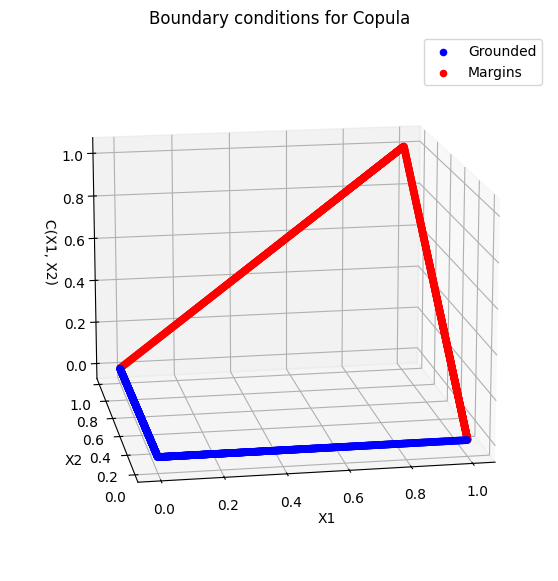
\includegraphics[width=0.5\linewidth]{3Theory/pictures/MarginsAndGrounded.png}
    \caption{Illustration showing what it means for a function to be grounded and to have margins.}
    \label{fig:GroundedAndMargins}
\end{figure}

Now we can formally define what a copula is. This is done as in \citet[p.~10]{Nelsen2006} in \Cref{def:copula}.
\begin{definition}\label{def:copula}
            \textbf{Copula in 2 dimensions}\\
            Equivalently, a copula is a function $C$ from $\mathrm{I}^2=[0,1]^2$ to $\mathrm{I} = [0,1]$ with the following properties:
            \begin{enumerate}
                \item For every $u, v \in \mathrm{I}$,
                \begin{align*}
                    C(u,0) &= C(0,v) = 0,\\
                    C(u,1) &= u, \; \mathrm{and } \; C(1,v) = v;
                \end{align*}
                \item For every $u_1, u_2, v_1, v_2 \in \mathrm{I}$ such that $u_1 \leq u_2$ and $v_1 \leq v_2$,
                \begin{align*}
                    C(u_2,v_2) - C(u_2,v_1) - C(u_1,v_2) + C(u_1,v_1) \geq 0.
                \end{align*}
            \end{enumerate}
\end{definition}

So, to describe what a copula is in simpler terms, it is a \gls{CDF} capturing the dependence between points on the probability space, obtained by performing the \gls{PIT} on each marginal distribution. 

A fundamental theorem connected to copulas is described in \Cref{the:Sklars}, as formulated by \citet[p.~18]{Nelsen2006}. 
\begin{theorem}\label{the:Sklars}
        \textbf{Theorem: Sklar's theorem} \\
        Let $H$ be a joint distribution function with margins $F$ and $G$ then there exists a copula $C$ such that for all $x,y \in \bar{\mathbf{R}} = \left[-\infty, \infty \right]$, 
        \begin{align}
            H(x,y) = C(F(x), G(y)). \label{eq:Sklar}
        \end{align}
        If $F$ and $G$ are continuous, then $C$ is unique; otherwise, $C$ is uniquely determined on $\mathrm{Ran}(F)\times\mathrm{Ran}(G)$. Conversely, if $C$ is a copula and $F$ and $G$ are distribution functions, then the function $H$ is a joint distribution function with margins $F$ and $G$.
\end{theorem}

\Cref{fig:CDFtoCopula} illustrates the correspondence, given in \Cref{eq:Sklar}, between a bivariate normal \gls{CDF} and its corresponding copula function. The copula has the same function value as the \gls{CDF} in each point where the mapping of points in $X_1\times X_2$ to $[0,1]\times[0,1]$ is done by the \gls{PIT}. The left picture shows the joint \gls{CDF} on the $\bar{R}^2$ domain. The right picture shows the corresponding copula function which lives in probability space. Hence, the difference between the joint \gls{CDF} and the copula is that the copula only exists on the unit square. 

\begin{figure}
    \centering
    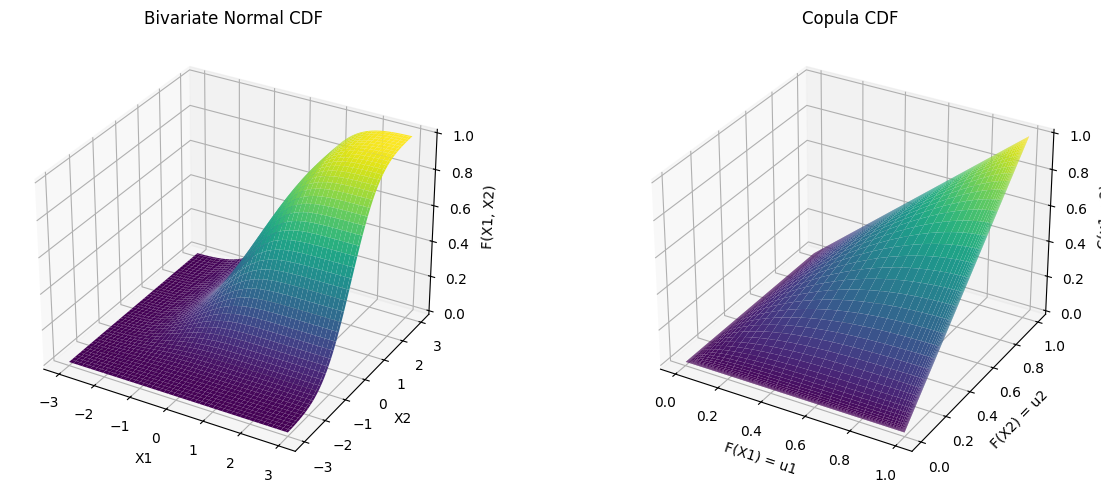
\includegraphics[width=1\linewidth]{3Theory/pictures/Copula.png}
    \caption{Illustration showing the correspondence between a bivariate normal \gls{CDF} and its corresponding copula function.}
    \label{fig:CDFtoCopula}
\end{figure}
\todo{fix Picture so that it isn't cut}

Sometimes it can be more convenient to write the \Cref{eq:Sklar} theorem in terms of the marginal probabilities $u_i$ rather than the marginal distributions $x_i$. It can be done by utilizing that $F_i(x_i) = u_i$ and $F_i^{-1}(u_i)= x_i$ so that 
\begin{align*}
    H(F_1^{-1}(u_1),F_2^{-1}(u_2))=H(x_1,x_2) = C(F_1(x_1), F_2(x_2))= C(u_1, u_2).
\end{align*}

Another important result for copulas is that they are translation invariant, the meaning of this is presented in \Cref{the:TranslationInvariance}, as done by \citet[p.~25]{Nelsen2006}.

\begin{theorem}\label{the:TranslationInvariance}
        \textbf{Theorem: Translation Invariance}\\
        Let $X$ and $Y$ be continuous random variables with copula $C_{X, Y}$. If $\alpha$ and $\beta$ are strictly increasing on $Ran(X)$ and $Ran(Y)$, respectively, then $C_{\alpha(X),\beta(Y)}  = C_{X,Y}$. Thus $C_{X, Y}$ is invariant under strictly increasing transformations of $X$ and $Y$.
\end{theorem}

From the requirements for a function to be a copula given in the definition of a copula in \Cref{def:copula} one can obtain bounds for how a copula can look. These bounds are defined as in \Cref{thm:FrechetBounds}.
    
\begin{theorem}\label{thm:FrechetBounds}
    \textbf{Fréchet-Hoeffding bounds} (\citet[p.~7]{Schmidt2006} or \citet[p.~11]{Nelsen2006})
    Consider a copula $C(\mathbf{u}) = C(u_1,u_2)$. Then the $C$ is bounded by
    \begin{align*}
        L(u_1,u_2) &\leq C(u_1,u_2) \leq U(u_1,u_2),\; \mathrm{ where}\\
        L(u_1,u_2) &= (u_1+u_2-1)^+\\
        U(u_1,u_2) &= \mathrm{min}(u_1,u_2).
    \end{align*}
    $L$ and $U$ are referred to as the Fréchet-Hoeffding lower and upper bounds respectively. 
\end{theorem}

Another important copula is the \emph{independence copula} or product copula corresponding to when the two marginal distributions are independent. The independence copula is defined by (\citet[p.~712]{BrigoMercurio2006} or \citet[p.~7]{Schmidt2006}) as
\begin{align*}
    \Pi(u_1,u_2) = u_1u_2.
\end{align*}

\Cref{fig:FrechetBounds} illustrates the upper (left) and lower (middle) bounds for copulas. We can think of it as if these bounds define a space where all copulas must be confined. One such copula is the independence copula (right) corresponding to the case when random variables are independent. 

\begin{figure}
    \centering
    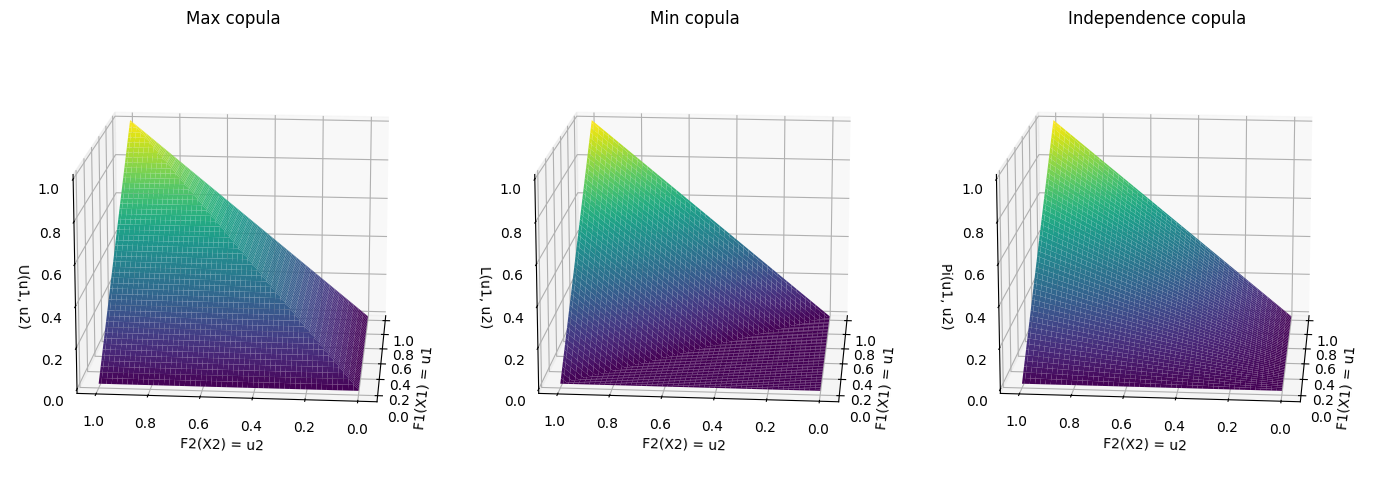
\includegraphics[width=1.\linewidth]{3Theory/pictures/FrechetBounds.png}
    \caption{Illustration of the Fréchet-Hoeffding upper $U$ (left), and lower $L$ (middle) bounds, as well as the independence copula $\Pi$ (right).}
    \label{fig:FrechetBounds}
\end{figure}

We have now discussed what copula functions are and arrived at that copulas are \gls{CDF}s on the unit square. When fitting copulas to data using \gls{MLE} it is often useful to have the copula \gls{PDF}. Deriving the copula \gls{PDF} is not as straightforward as one might initially think. Therefore we will derive the copula \gls{PDF} in the general case. Let $C(u_1,u_2)$ be the cpula \gls{CDF} you want to derive the \gls{PDF} for. The copula \gls{PDF} is defined as the second derivative of the copula \gls{CDF} with respect to $u_1$ and $u_2$.
\begin{align*}
    c(u_1,u_2) = \frac{\partial^2C(u_1,u_2)}{\partial u_1\partial u_2} = 
    \frac{\partial^2F(F_1^{-1}(u_1),F_2^{-1}(u_2))}{\partial u_1\partial u_2}
    = \\ f(F_1^{-1}(u_1),F_2^{-1}(u_2)) \frac{d}{du_1} F_1^{-1}(u_1)  \frac{d}{du_2} F_2^{-1}(u_2),
\end{align*}
where it can be shown that 
\begin{align*}
    \frac{d}{du_i} F_i^{-1}(u_i) = \frac{1}{f_i(F_i^{-1}(u_i))}.
\end{align*}
In the above equations, $F_i$ is the i:th marginal distribution function, \gls{CDF}, and $f_i$ is the marginal density function \gls{PDF}, $F$ is the joint distribution function.   

Hence the copula \gls{PDF} can be written as 
\begin{align*}
    c(u_1,u_2) &= f(F_1^{-1}(u_1),F_2^{-1}(u_2)) \frac{1}{f_1(F_1^{-1}(u_1))}\frac{1}{f_2(F_2^{-1}(u_2))}. 
\end{align*}

It can also be useful to write the copula in terms of data points that in the return space as this is typically where the data is observed
\begin{align*}
    c(u_1,u_2) &= f(F_1^{-1}(u_1),F_2^{-1}(u_2)) \frac{1}{f_1(F_1^{-1}(u_1))}\frac{1}{f_2(F_2^{-1}(u_2))},
\end{align*}
where $x_i = F_i^{-1}(u_i)$ and $f_i$ is the marginal \gls{PDF} of the i:th marginal distribution. \todo{How should we write the above equation?}



%%%%%%%%%%%%%%%%%%%%%%%%%%%%%%%%%%%%%%%%%%%%%%%%%%%%%%%%%%%%%%%%%%%%%%%%%%%%
%%%% The need for copulas
%%%%%%%%%%%%%%%%%%%%%%%%%%%%%%%%%%%%%%%%%%%%%%%%%%%%%%%%%%%%%%%%%%%%%%%%%%%%
\subsubsection{Usefulness of copulas}

The following examples are to illustrate how correlation can fail to capture the true dependence between random variables. The first example shows how correlation fails to capture the dependence between two random variables that are dependent but uncorrelated. The second example shows how correlation underestimates the true dependence between two random variables that are dependent but not normally distributed. This is to illustrate how copulas can be a better alternative to correlation when measuring dependence between random variables.

\begin{example}\label{ex:CorrelationFail}
    \textbf{Dependence is not always captured by correlation} \Citet[p.~21]{Danielsson2011} \\
    Let $X$ be a random variable such that, $X \sim N(0,1)$. Obviously, $X$ and $X^2$ are dependent. The covariance, $\mathrm{Cov}(X,X^2)$ is 
    \begin{align*}
        \mathrm{Cov}(X,X^2) &= E \left[  (X-E\left[  X \right])(X^2-E\left[  X^2 \right])  \right]\\
         &=  E \left[  (X)(X^2-1)  \right]\\
         &= E \left[  X^3  \right] - E \left[  X  \right]\\
         &= 0-0 = 0 .
    \end{align*}
    Since $\mathrm{Cov}(X,X^2) = \rho_{X,X^2}\sigma_{X}\sigma_{X^2} = \rho_{X,X^2}$ this shows that $\rho_{X,X^2} = 0.$
    Hence, $X$ and $X^2$ are dependent but uncorrelated. This shows how correlation falls short as a method of capturing non-linear dependence.
    %\todo{Maybe illustrate how this problem is solved using a copula(example of how in Brigo)}
    
    Using a copula instead we get
    \begin{align*}
    F_{X^2}(X^2) &= P(X^2 \leq x^2)\\
    &= P(\sqrt{X^2} \leq \sqrt{x^2})\\
    &= P(|X| \leq |x| )\\    
    &=P(X\leq x) = U2 \neq U1.\\
    \end{align*}

    Since the absolute value signs information is lost and hence 
    \begin{align*}
        P(U_1\leq u1, U_2\leq u2) = P(U_1\leq u1, U_1\leq u2) = \min(u_1,u_2).
    \end{align*}
    
\end{example}

\begin{example}
    Let $X$ be a random variable such that, $X \sim N(0,1)$. Obviously, $X$ and $e^X$ are dependent. The covariance, $\mathrm{Cov}(X,e^X)$ is
    \begin{align*}
        \mathrm{Cov}(X,e^X) &= E \left[  (X-E\left[  X \right])(e^X-E\left[  e^X \right])  \right]\\
         &=  E \left[  X(e^X-E\left[  e^X \right]) \right]\\
         &= E \left[  Xe^X  \right] - E \left[  X E \left[  e^X \right] \right]\\
         &= E \left[  Xe^X  \right]\\
         &= \int_{-\infty}^\infty xe^x \frac{1}{\sqrt{2\pi}} e^{\frac{-x^2}{2}} dx\\ %by definition of expectation for Cont. rand. var. 
         &=  \int_{-\infty}^\infty \frac{1}{\sqrt{2\pi}} x  e^{x -\frac{x^2}{2}} dx \\
         &= \int_{-\infty}^\infty \frac{1}{\sqrt{2\pi}} x  e^{-\frac{1}{2}(x-1)^2+\frac{1}{2} } dx \\
         &= \frac{e^\frac{1}{2}}{\sqrt{2\pi}}\int_{-\infty}^\infty x  e^{-\frac{1}{2}(x-1)^2 } dx\\
         & \mathrm{Let\;} u = x-1 \; \mathrm{then\;} x = u+1\\
         &= \frac{e^\frac{1}{2}}{\sqrt{2\pi}}\int_{-\infty}^\infty (u+1)e^{\frac{-u^2}{2}} du\\
         &= \frac{e^\frac{1}{2}}{\sqrt{2\pi}} \left( \int_{-\infty}^\infty ue^{\frac{-u^2}{2}}du +\int_{-\infty}^\infty e^{\frac{-u^2}{2}} du  \right) \\
         &= \frac{e^\frac{1}{2}}{\sqrt{2\pi}}\sqrt{2\pi}   \\
         &= e^{\frac{1}{2}}.\\
    \end{align*}
    If dividing with the standard deviations of $X$ and $e^X$ we get the correlation. To do this we need to calculate the variances of $X$ and $e^X$. We know that $\mathrm{Var}(X) = 1$ but need to calculate the variance of $e^X$. The variance of $e^X$ is calculated as
    \begin{align*}
        \mathrm{Var}(e^X) &= E[e^{2X}] - E[e^X]^2\\
        &= e^2 - e.\\
    \end{align*}
    The correlation is then calculated as
    \begin{align*}
        \mathrm{corr}(X,e^X) &= \frac{\mathrm{cov}(x,e^X)}{\sqrt{\mathrm{var}(x)} \sqrt{\mathrm{var}(e^X)}}\\
        & = \frac{e^{\frac{1}{2}}}{1\sqrt{e^2-e}}\\
        &=\sqrt{\frac{1}{e-1}} \approx 0.76. 
    \end{align*}
    If instead using the copula to calculate the correlation we can see that the correlation is not capturing the true dependence between $X$ and $e^X$. To see this we can use the \gls{PIT} to transform $X$ and $e^X$ into uniform random variables. If we let $F_X(X)=U_1$ be the normal data transformed to uniform random variables and $F_{e^X}(e^X)=U_2$ be the log-normal data transformed to uniform random variables we can see that 
    \begin{align*}
        F_{e^X}(e^X) &= P(e^X \leq e^x)\\
        &= P(\ln(e^X) \leq \ln (e^x))\\
        &=P(X\leq x) = U2 = U1.\\
    \end{align*}
    Since $U_1 = U_2$ we have 
    \begin{align*}
        P(U_1\leq u1, U_2\leq u2) = P(U_1\leq u1, U_1\leq u2) = \min(u_1,u_2).
    \end{align*}
    This is the upper copula given by the upper Fréchet-Hoeffding bound, which is the copula corresponding to the correlation being one. Hence, correlation underestimates  the true dependence between the random variables. Showing how copulas can capture dependence when correlation fails. 

    \begin{generalinstructions}
        Would be nice to tie this to something in finance. Such as the relationship between stocks returns and derivative prices.

        This shows that estimating the correlation in a setting when the different marginals are not both normal can be misleading. This is a problem in finance where one often uses correlation to estimate the dependence between different assets. This is especially true when using correlation to estimate the dependence between stocks and derivatives.
    \end{generalinstructions}


\end{example}
    
\begin{figure}
    \label{fig:ExamplePlots}
    \centering
    \begin{minipage}{0.4\textwidth}
        \centering
        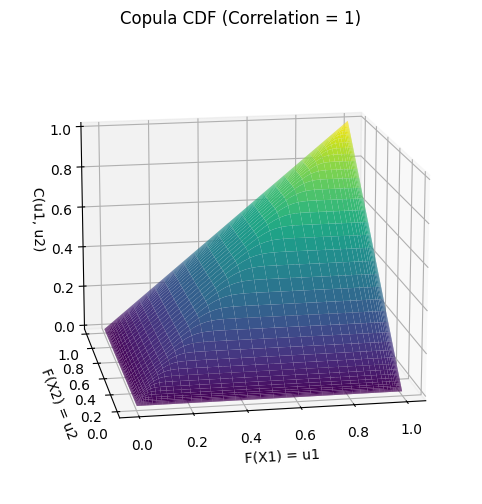
\includegraphics[width=\textwidth]{3Theory/pictures/TrueCopulaExponential.png}
        \subcaption{}
    \end{minipage}
    \hfill
    \begin{minipage}{0.4\textwidth}
        \centering
        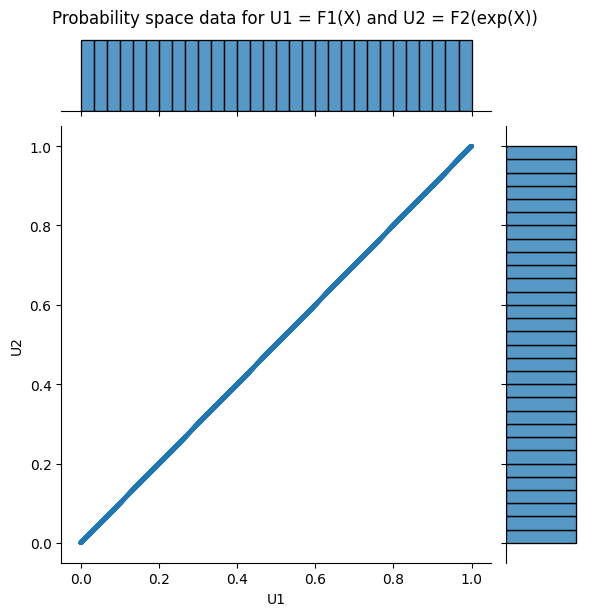
\includegraphics[width=\textwidth]{3Theory/pictures/exponentialDependenceScatterProb.png}
        \subcaption{}
    \end{minipage}
    \vfill
    \begin{minipage}{0.4\textwidth}
        \centering
        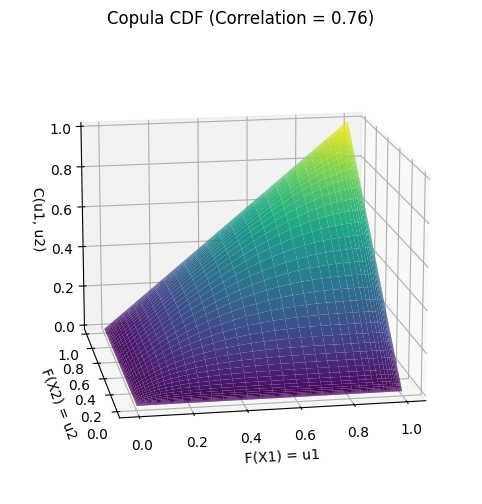
\includegraphics[width=\textwidth]{3Theory/pictures/CorrelationEstimationExponential.png}
        \subcaption{}
    \end{minipage}
    \hfill
    \begin{minipage}{0.4\textwidth}
        \centering
        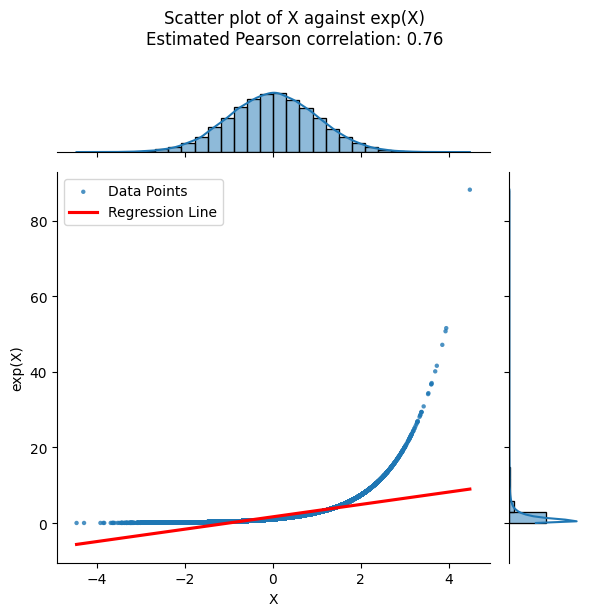
\includegraphics[width=\textwidth]{3Theory/pictures/exponentialDependenceScatterRet.png}
        \subcaption{}
    \end{minipage}
    \caption{.}
\end{figure}

Up to now we have not yet provided an example of the usefulness of copulas. The next section will show an example of how copulas are useful in practice.

%%%%%%%%%%%%%%%%%%%%%%%%%%%%%%%%%%%%%%%%%%%%%%%%%%%%%%%%%%%%%%%%%%%%%%%%%%%%
%%%% Use for copula
%%%%%%%%%%%%%%%%%%%%%%%%%%%%%%%%%%%%%%%%%%%%%%%%%%%%%%%%%%%%%%%%%%%%%%%%%%%%
\subsubsection{Usecase for copula in practice}\label{sec:CopulaUseCase}
If there are several sources of randomness present in a system where monte carlo methods are used, potential dependence between the sources of randomness has to be taken into account. Copulas are a powerful tool for modeling the dependence structure between random variables. They allow for separation of the dependence and the marginal distributions. By using copulas, we can generate samples from multivariate distributions with specified marginals and a desired dependence structure by generating dependent marginally distributed uniform random numbers. These are then transformed to the desired marginal distributions using the inverse of the marginal \gls{CDF}s by the inverse transform method \Cref{def:InverseTransformMethod}.

Let $U = (U_1,U_2)$ be a point specified by two marginally uniformly distributed random variables $U_1$ and $U_2$ sampled from a copula giving them some dependence. Then random numbers $X = (X_1,X_2)$ with the dependence specified by the copula and desired marginal distributions can be generated by transforming the uniform random numbers using the \gls{ITM}. This is done by using the inverse of the marginal \gls{CDF}s as follows
\begin{align*}
    X_1 = F_1^{-1}(U_1); \\
    X_2 = F_2^{-1}(U_2).
\end{align*}

The usefulness of copulas in sampling is visualised in \Cref{fig:CopulaSampling}. The left figure shows a sample from a Clayton copula with $\alpha = 4$. The right figure shows the same sample after applying the \gls{ITM} using a standard normal distribution for each marginal. Note that the \gls{ITM} can be applied to each of the dimensions of the copula data thanks to the fact that copulas by definition have uniform marginals. 

\begin{figure}[h]
    \centering
    \begin{subfigure}[t]{0.45\linewidth}
        \centering
        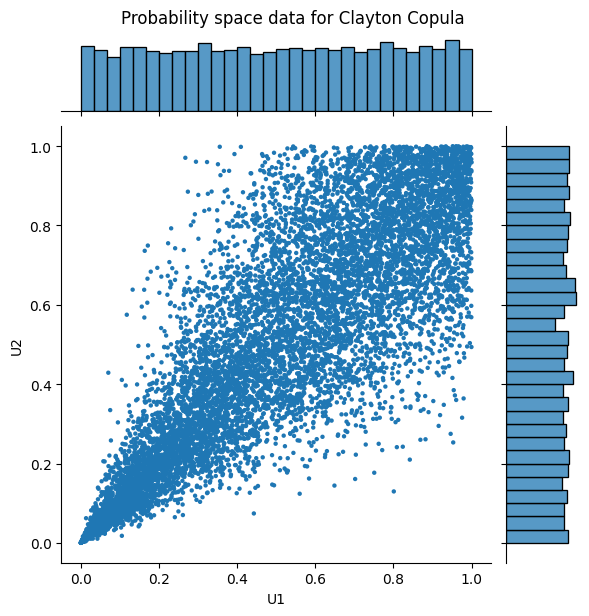
\includegraphics[width=\linewidth]{3Theory/pictures/ProbabilitySpaceClayton.png}
        \caption{Sample from a Clayton copula with $\alpha = 4$. } 
        \label{fig:ProbabilitySpaceDataClayton}
    \end{subfigure}
    \hfill
    \begin{subfigure}[t]{0.45\linewidth}
        \centering
        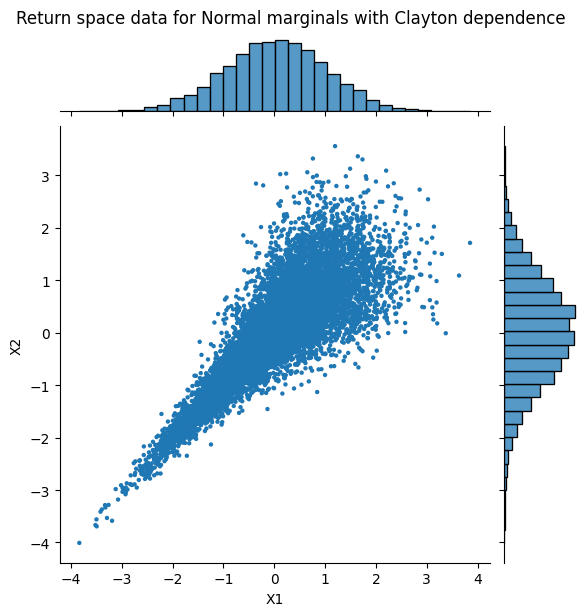
\includegraphics[width=\linewidth]{3Theory/pictures/ReturnSpaceDataClayton.png}
        \caption{Sample from Clayton copula after applying the inverse transform method using a standard normal distribution.}
        \label{fig:ReturnSpaceDataClayton}
    \end{subfigure}
    \caption{Illustration of sampling from a clayton copula with standard normal marginal distributions.}
    \label{fig:CopulaSampling}
\end{figure}


In the above example we have seen the usefulness of copulas in sampling. The example does not go into the nontrivial task of sampling from a copula. Therefore the next section introduces conditional sampling which is a method of sampling from a copula. 

\subsubsection{Conditional sampling from copulas}\label{sec:ConditionalSampling} from \Citet[p.~41]{Nelsen2006}\\
For some copulas samples can be generated using conditional sampling which works as follows. First, we generate two independent uniform random numbers $z_1,z_2 \sim \mathrm{Unif}(0,1)$. 
The first random number is calculated without respect for the second random number hence we set $u_2 =1$. We want to solve
\begin{align*}
    C(u_1,u_2) =z_1,
\end{align*}
for $u_1$ independently of $u_2$. 

By using that the copula is a \gls{CDF} and can be written as a probability we can see that 
\begin{align*}
    C(u_1,u_2) = P(U_1\leq u_1, U_2\leq u_2) = P(U_1\leq u_1,U_2 \leq 1) = P(U_1\leq u_1).
\end{align*} 
Since $u_2 = 1$ no constraint is enforced on $U_2$. By the definition of a copula we have that 
\begin{align*}
    C(u_1,1) = u_1 = z_1.
\end{align*}
So we set the first random number as $u_1 = z_1$.

The second random number is obtained by computing the conditional copula \gls{CDF} given the first random number. This is done by using the conditional copula \gls{CDF} defined as
\begin{align*}
    C_{2|1}(u_2|u_1) = \frac{\partial C(u_1,u_2)}{\partial u_1}.
\end{align*}
To compute the second random number we need to solve the equation
\begin{align*}
    C_{2|1}(u_2|u_1) = z_2,
\end{align*}
for $u_2$. That is
\begin{align*}
    u_2 = C^{-1}_{2|1}(z_2|z_1).
\end{align*}
The pair $(u_1,u_2)$ is now a sample from the copula. The method can be repeated to generate more samples from the copula.

\todo{$C^{-1}$ is the quasi inverse since copula can be flat} 

\todo{Acceptance rejection sampling  }


%%%%%%%%%%%%%%%%%%%%%%%%%%%%%%%%%%%%%%%%%%%%%%%%%%%%%%%%%%%%%%%%%%%%%%%%%%%%
%%%% Other Copulas
%%%%%%%%%%%%%%%%%%%%%%%%%%%%%%%%%%%%%%%%%%%%%%%%%%%%%%%%%%%%%%%%%%%%%%%%%%%%
\subsection{Other copulas}
This section introduces some of the most commonly used copulas. Some copulas are defined through known statistical distributions such as the Gaussian copula and the Student's t copula. Another type of copulas is the family of Archimedean copulas, of which the Clayton copula is an example.

%%%%%%%%%%%%%%%%%%%%%%%%%%%%%%%%%%%%%%%%%%%%%%%%%%%%%%%%%%%%%%%%%%%%%%%%%%%%
%%%% Gaussian Copula
%%%%%%%%%%%%%%%%%%%%%%%%%%%%%%%%%%%%%%%%%%%%%%%%%%%%%%%%%%%%%%%%%%%%%%%%%%%%
\subsubsection{Gaussian Copula}\label{sec:GaussianCopula}
A commonly used copula is the Gaussian copula which is derived from the centered multivariate normal distribution. 

Let $\boldsymbol{\Phi}_\Sigma(x_1,x_2)$ be the bivariate normal distribution \gls{CDF} with correlation matrix $\Sigma$. Let $\Phi(x)$ be the univariate normal \gls{CDF}. Then the Gaussian copula is defined, as in \citet[p.~112]{Umberto2004copulaMethods}  by 
\begin{align*}
    C_\Sigma(u_1,u_2) = \boldsymbol{\Phi}_\Sigma(\Phi^{-1}(u_1),\Phi^{-1}(u_2)).
\end{align*}

In the above expression $\Sigma$ is the correlation matrix in two dimensions 
\begin{align*}
    \Sigma = 
    \begin{bmatrix}
            1 & \rho_{1,2} \\
            \rho_{1,2} & 1
    \end{bmatrix},
\end{align*}
so in the sequel when $\rho$ is used it refers to $\rho_{1,2}$ in the correlation matrix.

The copula function, which is a \gls{CDF} can be expressed on integral form as done by \citet[p.~112]{Umberto2004copulaMethods}
\begin{align*}
     C_{\Sigma} (u_1,u_2)
    = \int_{-\infty}^{\Phi^{-1}(u_1)}\int_{-\infty}^{\Phi^{-1}(u_2)}
    \frac{1}{2\pi\sqrt{1-\rho^2}} \mathrm{exp}\left\{ - \frac{s^2-2\rho st+t^2}{2(1-\rho^2)}   \right\} dsdt.
\end{align*} 

The \gls{PDF} of the Gaussian copula function can be shown to be 
\begin{align*}
     c_{\Sigma} (u_1,u_2)
    = \frac{1}{\sqrt{1-\rho^2}} \mathrm{exp}\left\{  \frac{-2\rho^2\Phi^{-1}(u_1)^2  +2\rho \Phi^{-1}(u_1)\Phi^{-1}(u_2) -2\rho^2\Phi^{-1}(u_2)^2}{2(1-\rho^2)}   \right\},
\end{align*}
as stated in \citet[p.267]{Alexander2008}.



\textbf{Fitting}(alternative source: \Citet[pp.~281-283]{Alexander2008})
To fit the Gaussian copula to data we need to compute the correlation matrix $\Sigma$. This is done by first estimating the sample covariance matrix and then normalizing it to obtain the correlation matrix \Citet[p.~523]{SAS2014}. 

\textbf{Sampling}(alternative source: \Citet[p.~19]{Schmidt2006})
To sample from a Gaussian copula we can first generate a sample from the multivariate normal distribution with the desired correlation matrix $\Sigma$. This is done by multiplying a standard normal random vector with the Cholesky decomposition of the correlation matrix. The Cholesky decomposition can be thought of as a matrix square root of the correlation matrix. The resulting sample of correlated random numbers is then transformed to uniform random numbers using the \gls{PIT}. This is done by applying the univariate normal \gls{CDF} to each of the elements in the sample. The resulting sample is then a sample from the Gaussian copula \Citet[p.~523]{SAS2014}.



%%%%%%%%%%%%%%%%%%%%%%%%%%%%%%%%%%%%%%%%%%%%%%%%%%%%%%%%%%%%%%%%%%%%%%%%%%%%
%%%% Students Copula
%%%%%%%%%%%%%%%%%%%%%%%%%%%%%%%%%%%%%%%%%%%%%%%%%%%%%%%%%%%%%%%%%%%%%%%%%%%%
\subsubsection{Students t Copula}\label{sec:StudentsCopula} \citet[p.~116]{Umberto2004copulaMethods} 
The Student's $t$ copula can be defined similarly to the Gaussian copula above. We denote the Student's $t$ copula by 
\begin{align*}
    C_{\nu,\Sigma}(u_1,u_2) = \boldsymbol{t}(t_\nu^{-1}(u_1),t_\nu^{-1}(u_1)),
\end{align*}
as done by \citet[p.~268]{Alexander2008}, where $\nu >0$ is the degrees of freedom, $\boldsymbol{t}$ is the multivariate Student's $t$ distribution, $t$ is the univariate Student's $t$ distribution, and $\Sigma$ is the correlation matrix matrix.

The Student's $t$ copula \gls{CDF} is 
\begin{align*}
     C_{\nu,\Sigma}^t (u_1,u_2)
    = \int_{-\infty}^{t_\nu^{-1(u_1)}}\int_{-\infty}^{t_\nu^{-1(u_2)}}
    \frac{1}{2\pi\sqrt{1-\rho^2}} \left\{  1+ \frac{s^2-2\rho st+t^2}{\nu(1-\rho^2)}   \right\} dsdt,
\end{align*}
as defined by \citet[p.~116]{Umberto2004copulaMethods}. The corresponding copula \gls{CDF} is, by the same logic as for the Gaussian case, the integrand in the expression above times the two partial derivatives of the marginal distributions. The resulting expression for the copula \gls{PDF} $c_{\nu,\rho}$ is therefore 
\begin{align*}
    c_{\nu,\Sigma}(u_1,u_2) = \frac{\Gamma(\frac{\nu+2}{2})\Gamma(\frac{\nu}{2})\prod_{j=1}^2\left( 1+ \frac{t_\nu^{-1}(u_j)^2}{\nu}\right)^{\frac{\nu+2}{2}} } {\sqrt{\rho} \;\Gamma(\frac{\nu+1}{2})^{2}\left( 1+ \frac{t_\nu^{-1}(u_1)^2 + t_\nu^{-1}(u_2)^2 -2\rho t_\nu^{-1}(u_1) t_\nu^{-1}(u_2) }{\nu(1-\rho^2)}\right)},
\end{align*}
as stated by \citet[p.~117]{Umberto2004copulaMethods}.
\todo{Say what gamma is}

\textbf{Fitting} 
To fit the Student's $t$ copula to data we need to compute the correlation matrix $\Sigma$ and the degrees of freedom $\nu$. It is common to first estimate the correlation matrix and then estimate the degrees of freedom using \gls{MLE} \Citet[p.~283]{Alexander2008}.  
\todo{They often say to use either spearman or kendal here. does it matter? }

\textbf{Sampling} (alternative source: \Citet[p.~19]{Schmidt2006})
Sampling from a Student's $t$ copula is similar to sampling from a Gaussian copula. First, we generate a sample from the multivariate Student's $t$ distribution with the desired correlation matrix $\Sigma$ and degrees of freedom $\nu$. This can be done by generating a sample $Z$ from a normal distribution with correlation matrix $\Sigma$ as described for the Gaussian copula. These normal random numbers can then be transformed into Student's $t$ distributed sample $X$ by the calculation $X = Z\sqrt{\frac{\nu}{s}} $, where s is a sample from a $\chi^2$ distribution with $\nu$ degrees of freedom. The resulting sample of correlated Student's $t$ random numbers is then transformed to uniform random numbers using the \gls{PIT}. This is done by applying the univariate Student's $t$ \gls{CDF} with $\nu$ degrees of freedom to each of the elements in the sample. The resulting sample is then a sample from the Student's $t$ copula \Citet[p.~524]{SAS2014}. 

%%%%%%%%%%%%%%%%%%%%%%%%%%%%%%%%%%%%%%%%%%%%%%%%%%%%%%%%%%%%%%%%%%%%%%%%%%%%
%%%% Clayton Copula
%%%%%%%%%%%%%%%%%%%%%%%%%%%%%%%%%%%%%%%%%%%%%%%%%%%%%%%%%%%%%%%%%%%%%%%%%%%%
\subsubsection{Clayton Copula}\label{sec:ClaytonCopula}
Archimedian copulas have the general expression  
\begin{align*}
    C(u_1,u_2) = \Psi^{-1}(\Psi(u_1),\Psi(u_2)),
\end{align*}
for some generator function $\Psi$, as defined by \citet[p.~150]{Umberto2004copulaMethods}.

The Clayton copula, which is one instance of an Archimedean copula, uses the generator function
\begin{align*}
    \Psi(u) &=u^{-\alpha}-1, \\
\end{align*}
and its inverse
\begin{align*}
    \Psi^{-1}(x) &= (x+1)^{\frac{-1}{\alpha}},
\end{align*}
where $\alpha > 0$. 

This gives the bivariate Clayton copula \gls{CDF}
\begin{align*}
    C(u_1,u_2) = (u_1^{-\alpha} + u_2^{-\alpha}-1)^{\frac{-1}{\alpha}}.
\end{align*}

The Clayton copula \gls{PDF} is 
\begin{align*}
    c(u_1,u_2) = (\alpha+1)(u_1^{-\alpha}+u_2^{-\alpha}-1)^{-2- \frac{1}{\alpha}}u_1^{-\alpha -1} u_2^{-\alpha -1},
\end{align*}
as stated by \citet[p.~272]{Alexander2008}. 

\textbf{Fitting}\Citet[pp.~281-283]{Alexander2008}
Fitting the Clayton copula to data is done by estimating the parameter $\alpha$. This is done by using \gls{MLE} with the copula \gls{PDF} as the terms in the sum of the log likelihood function. \gls{MLE} applied to copula fitting is described in \Citet[p.~2]{Choros2010}. 

\textbf{Sampling}
To sample from a Clayton copula we can use conditional sampling as described in \Cref{sec:ConditionalSampling}. It is convenient to sample from because there is an analytical expression for the Copula from which the conditional copula can be derived. 


%%%%%%%%%%%%%%%%%%%%%%%%%%%%%%%%%%%%%%%%%%%%%%%%%%%%%%%%%%%%%%%%%%%%%%%%%%%%
%%%% Correlation measures
%%%%%%%%%%%%%%%%%%%%%%%%%%%%%%%%%%%%%%%%%%%%%%%%%%%%%%%%%%%%%%%%%%%%%%%%%%%%
\subsubsection{Correlation measures}
\textbf{Keep this part until I decide if I will go deeper into this.}
(in Market risk analysis p.280 and p.256)
Denote the correlation measure as $\hat{\rho}$

\textbf{Pearson correlation}
for Pearson correlation
$\hat{\rho} = \rho_p$

\textbf{Spearman correlation}
For Spearman rho $\rho_s$:
\begin{align*}
    \rho_s = 1-\frac{6D}{n(n^2-1)},\; \mathrm{where} \; D=\sum_ {i=1}^nd_i^2.
\end{align*}

$\hat{\rho} =2\mathrm{sin} \big ( \frac{\pi}{6}\rho_p \big)$

\textbf{Kendals Tau}
For Kendals Tau $\tau$:
\begin{align*}
    \tau = \frac{N_c-N_d}{\frac{1}{2}n(n-1)}
\end{align*}
where $N_c$ and $N_d$ are the numbers of concordant and discordant pairs respectively.
$\hat{\rho} = \mathrm{sin}\big(\frac{\pi}{2}\tau \big) $
\todo{Maybe remove}

%%%%%%%%%%%%%%%%%%%%%%%%%%%%%%%%%%%%%%%%%%%%%%%%%%%%%%%%%%%%%%%%%%%%%%%%%%%%
%%%% neural networks
%%%%%%%%%%%%%%%%%%%%%%%%%%%%%%%%%%%%%%%%%%%%%%%%%%%%%%%%%%%%%%%%%%%%%%%%%%%%
\subsection{Neural Networks}
A full introduction of \gls{NN}s is outside the scope of this thesis. Despite other simpler topics being thoroughly explained, in those cases that has been to explain what something else is or to motivate some method. This section will only give a brief introduction to \gls{NN}s and how they can be used for unsupervised learning. In particular a short description of how to solve differential equations using \gls{NN}s as this will be used in the neural copula. For a more in-depth introduction to \gls{NN}s, see \todo{reference}.



\begin{generalinstructions}
    References to standard literature about NNs, training...

    Explain how NNs can be used to solve DE:s by defining a loss function in a clever way
\end{generalinstructions}





%%%%%%%%%%%%%%%%%%%%%%%%%%%%%%%%%%%%%%%%%%%%%%%%%%%%%%%%%%%%%%%%%%%%%%%%%%%%
%%%% Neural Copula
%%%%%%%%%%%%%%%%%%%%%%%%%%%%%%%%%%%%%%%%%%%%%%%%%%%%%%%%%%%%%%%%%%%%%%%%%%%%

\subsection{Neural Copula (Own model formulation )} \todo{Reference to paper}
A \gls{NC} is a method proposed to use a \gls{NN} to approximate a copula function. 


\subsubsection{Overall procedure}
The overall procedure when using a \gls{NC} is to fit one \gls{NN} approximating each marginal distribution. These functions and their derivatives are then used to calculate the copula function value and the copula \gls{PDF} function values 

transform the data in each data dimension to the $[0,1]$ domain via the \gls{PIT}. The resulting data points form data points that lie in probability space. These data points are then used for fitting a \gls{NN} approximating the copula function. 


\subsubsection{Data }
First, define the observed data as $x^{\mathrm{obs}}\in \mathbb{R}^2 $. To fit the marginal distributions, the data must be normalized to lie in the interval $\mathbb{I}^2 = [0,1]^2$. We normalize the data $x$ by using min max normalization defined as
\begin{align*}
    x_{i,j} = \frac{x_{i,j}^{\mathrm{obs}} - \min_i(x_{j}^{\mathrm{obs}})}{  \max_i(x_{j}^{\mathrm{obs}})- \min_i(x_{j}^{\mathrm{obs}})}.
\end{align*}
The normalized data $x$ is then used to fit a marginal distribution $\hat{F}_j$ to each dimension $x_j, \; \mathrm{where} \; j=\{1,2\}$ if $x$ has two dimensions. 


\subsubsection{Marginal model architecture}
A marginal distribution is fitted for each dimension of the data using a \gls{NN} having the following architecture 
\begin{align*}
    \mathrm{Input\;layer:} \; & \mathbf{h}_m^0 = x_j \in \Omega_j = \mathbb{I}; \\
    \mathrm{Hidden\;layer:} \; & \mathbf{h}_m^{k+1} = \mathrm{tanh}(\mathbf{w}_m^{k} \mathbf{h}_m^{k} + \mathbf{b}_m^{k}), \; k \in \{0,1, \dots, l_m -1 \};\\
    \mathrm{Output\;layer:} \; & \hat{F}_j = \mathrm{sigmoid}(\mathbf{w}_m^{l_m} \mathbf{h}_m^{l_m} + \mathbf{b}_m^{l_m}) \in \left[0,1 \right],
\end{align*}
where $\hat{F}_j$ is the estimated marginal \gls{CDF}, $\Omega$ is the entire domain where the data can be, $l_m$ is the number of layers in the network, $\mathbf{w}_m^{k}$ are the weights in the $k$th layer,  $\mathbf{h}_m^{k}$ is the input data in the $k$th layer, and $\mathbf{b}_m^{k}$ is the biases in the $k$th layer. Note that the weights, biases, and input data are different for each dimension in the data (maybe obvious, but for notations' sake). 

\subsubsection{Marginal loss function}\label{sec:NeuralMarginalLoss}
This section defines the loss function for a marginal model $\hat{F}_j$. First, we define the datasets that will be used for calculating the loss function. Let $D_{obs}$ be the set of observed data points $x_j$ for the $ j$th dimension of the data. Also, let $D_u$ be a set of uniformly distributed data points on the domain $\Omega$ of the data. Let $\hat{f}_j$ denote the \gls{PDF} corresponding to $\hat{F}_j$.

The loss function consists of four parts that are designed to ensure that the network fits the data as well as possible whilst following the requirements of a \gls{CDF}. The first part of the loss function maximizes the log likelihood of the fitted \gls{CDF} to the observed data. Since the network minimizes the loss during training, we need the negative log likelihood as the loss. The first part of the loss is defined as 
\begin{align*}
    L_1^m = \frac{-1}{|D_{obs}|} \sum_{i \in D_{obs}} \log(\hat{f}_j(x_i)).
\end{align*}

The second part of the loss function ensures that the \gls{PDF} is not negative. This corresponds to the loss function 
\begin{align*}
    L_2^m = \int_{x_{i\in\Omega}} (-\hat{f}(x))^+dx \approx \frac{-1}{|D_{u}|} \sum_{i \in D_{u}} (-\hat{f}_j(x_i))^+.
\end{align*}
The third part of the loss function ensures that the integral of $\hat{f}$ over $\Omega$ is one as stated in \cref{rem:pdfProperties}. The loss can be formulated as 
\begin{align*}
    L_3^m = \left | 1- \int_{x\in \Omega} \hat{f}(x) dx    \right | \approx \left | 1- \frac{1}{|D_{u}|} \sum_{i \in D_{u}} \hat{f}_j(x_i)  \right |.
\end{align*}
The final loss ensures that the \gls{CDF} begins at zero and ends at one. This is ensured by the loss
\begin{align*}
    L_4^m = \hat{F}_j(0) + |1- \hat{F}_j(1) |.
\end{align*}

The total loss can be formulated as a linear combination of the loss components. 
\begin{align*}
    L^m = \sum_{i=1}^4 \lambda_i L_i^m,
\end{align*}
where $\lambda_i$ is the weigh put on the $i$:th loss component. 

\subsubsection{Copula model architecture} \citet[pp.~9--11]{ZengWang2022}
The copula model $\hat{C}$ is defined as 
\begin{align*}
    \mathrm{Input\;layer:} \; & \mathbf{h}_c^0 = x \in \Omega^2 = \mathbb{I}^2; \\
    \mathrm{Hidden\;layer:} \; & \mathbf{h}_c^{k+1} = \mathrm{tanh}(\mathbf{w}_c^{k} \mathbf{h}_c^{k} + \mathbf{b}_c^{k}), \; k \in \{0,1, \dots, l_c -1 \};\\
    \mathrm{Output\;layer:} \; & \hat{C} = \mathrm{sigmoid}(\mathbf{w}_c^{l_c} \mathbf{h}_c^{l_c} + \mathbf{b}_c^{l_c}) \in \left[0,1 \right].
\end{align*}
\todo{Should i change $u$ and $x$ to bold since vectors? }

\subsubsection{Copula loss function}\label{sec:NeuralCopulaLoss}
Before defining the copula loss function, we need to define the different data sets used to compute the loss. Additionally, we need to define the copula \gls{CDF} and its corresponding copula \gls{PDF}. 

First, we define the datasets. Let $D_{\mathrm{obs}}$ be the observed data points $x \in \Omega_1\Omega_2  = \mathbb{I}^2$. Let $D_{u}$ be uniformly distributed data on $\mathbb{I}^2$. Let $D_{\bar{u}}$ be uniformly distributed points on the upper boundary of the unit square $\mathbb{I}^2$. Let $D_{\underline{u}}$ be a set of points uniformly distributed on the lower boundary of the unit square $\mathbb{I}$. In \Cref{fig:datasetsNC} the datasets used to train the \gls{NC} are visualized. Before explaining the picture, we ephasise that the data used here is in the $x$-space and not in the transformed space $u$ as one might think. The reason for this is the case is that it will be easier to write the copula \gls{PDF} in terms of $x$ than of $u$ as explained below. The blue data points are uniformly distributed over the upper boundaries of the region where one variable is one. The grey points are uniformly distributed on the lower boundaries of the region where one of the variables is zero. The red data points are the observed data. The black data points are uniformly distributed over the interval. 

\begin{figure}
    \centering
    \includegraphics[width=0.5\linewidth]{3Theory/pictures/DatasetsNC.png}
    \caption{The different datasets used for training the \gls{NC} visualized.}
    \label{fig:datasetsNC}
\end{figure}
\todo{See if red is right after rethinking}


The copula model itself approximates a copula function which is a \gls{CDF} on the unit square $\mathbb{I}^2$. Normally the copula function is denoted in terms of its uniform marginals $u$ consisting of $u_1$ and $u_2$. The copula function can be written in terms of the data points $x$ consisting of $x_1$ and $x_2$. 


\begin{align*}
    \hat{C}(u) = \hat{C}(u_1,u_2) = \hat{C}(\hat{F}_1(x_1),\hat{F}_2(x_2))= \hat{C}(x).
\end{align*}
The corresponding copula \gls{PDF} can be written as  
\todo{2nd half unnecessary?}
\begin{align*}
    \hat{c}(x) = \hat{c}(x_1,x_2) 
    = \frac{\partial^2 \hat{C}(\hat{F}_1(x_1),\hat{F}_2(x_2))}{\partial \hat{F}_1(x_1) \partial \hat{F}_2(x_2)} \hat{f}_1(x_1),\hat{f}_2(x_2))\\
    = \frac{\partial^2 \hat{C}(u_1,u_2)}{\partial u_1 \partial u_2} \hat{f}_1(\hat{F}_1^{-1}(u_1)) \hat{f}_2(\hat{F}_2^{-1}(u_2)) 
    = \hat{c}(u).
\end{align*}

\todo{These equations need to be checked. I think they are wrong. }


In the loss function, it is advantageous to have the copula \gls{CDF} and \gls{PDF} written in terms of $x$ rather than of $u$. This is because there is no mechanism for calculating the inverse of a \gls{NN}. The inverse is needed in order to write the copula \gls{PDF} in terms of $u$. However, as shown above, the copula \gls{PDF} can be written in terms of $x$ using the marginal \gls{CDF}s and \gls{PDF}s, removing the need for the inverse \gls{CDF}s.   

Now we are ready to introduce the copula loss function, which consists of five parts. The first part, as in the marginal model, maximizes the log likelihood and is defined as
\begin{align*}
    L_1^c = \frac{-1}{|D_{obs}|} \sum_{i \in D_{obs}} \log(\hat{c}(x_i)).
\end{align*}
The second term ensures positivity of the copula \gls{PDF} and is defined by
\begin{align*}
    L_2^c = \int_{x_1\in\Omega}\int_{x_2\in\Omega} (-\hat{c}(x))^+dx_1dx_2 \approx \frac{-1}{|D_{u}|} \sum_{i \in D_{u}} (-\hat{c}(x_i))^+.
\end{align*}
The third part ensures that the copula PDF integrates to one and is defined as
\begin{align*}
    L_3^c = \left | 1- \int_{x_1\in\Omega}\int_{x_2\in\Omega} \hat{c}(x_j) dx_1 dx_2   \right | \approx \left | 1- \frac{1}{|D_{\mathrm{u}}|^2} \sum_{i \in D_{u}} \hat{c}(x_i)  \right |.
\end{align*}
The fourth term is supposed to ensure that the copula function is grounded and that it has margins. It is defined as
\begin{align*}
    L_4^c = \sum_{i \in D_{\underline{u}}} \hat{C}(x_i) + \sum_{i \in D_{\bar{u}}} \left| \hat{C}(x_i) - \max(x_i) \right|.
\end{align*}
The fifth term  ensures that the copula is $2$-increasing and is defined as
\begin{align*}
    L_5^c = \frac{1}{|D_{u}|} \sum_{i \in D_{u}} \left| \hat{C}(x_i) - \frac{1}{|D_{\mathrm{obs}}|}\sum_{j\in D_{\mathrm{obs}}} \mathrm{flag}(x_i,x_j) \right|,
\end{align*}
where $\mathrm{flag(x,y)}$ is defined as 
\begin{align*}
    \mathrm{flag}(x,y) =  
    \begin{cases}
        1 \; \mathrm{if} \; \forall j \leq 2, y_j < x_j\\
        0 \; \mathrm{otherwise}.
    \end{cases}
\end{align*}
So the flag function compares two points $x$ and $y$ and gives back one if all dimensions $x$ is greater than $y$ in all dimensions. What this does it that for each point in $D_u$ the copula \gls{CDF} is compared to the fraction of points in $D_{obs}$ that are smaller than the point in $D_u$. This the value of the copula and the fraction should be similar if the data is 2-increasing.   

As for the marginal model, the total loss is given by a linear combination of the loss terms defined as follows
\begin{align*}
    L^c = \sum_{i=1}^5 \lambda_i L_i^c,
\end{align*}
where $\lambda_i$ is the weight assigned to each part loss term. 


\subsubsection{Fittig and sampling procedure}\label{sec:NeuralCopulaFittingAndSampling}
\textbf{Fitting}
In the neural copula article the fitting procedure is as follows: 
First the data is normalized to lie in the interval between zero and one using min-max normalization. The normalized data is then used to fit the \gls{NC} to data by first fitting marginal distributions to each dimension of the data. This is done by training \gls{NN}s that minimize the marginal loss function defined in \Cref{sec:NeuralMarginalLoss} for each dimension. The copula is fitted by training another \gls{NN} that minimizes the copula loss function defined in \Cref{sec:NeuralCopulaLoss}. 

\begin{generalinstructions}
    This method has a flaw when using it for risk applications. Firstly, in the article they use pure price data for training the model. This could be a problem since one is generally more interested in generating returns than prices in mathematical finance as described in \Cref{sec:MathematicalFinance}. I can acknowledge that one could argue that the copula should be invariant to strictly increasing transformations (this would require pluging copula random numbers into some other distributions that have not been fitted). However, this will cause problems when sampling from the copula. The reason for this is that the sampled data is bounded by the largest and smallest observed values in the training data. This means that the sampled price data will be confined to the interval in the training data, which does not reflect the usual development of price data. As an example, think about a stock at all time high where one wants to generate potential future observations. The simulated prices can only be lower than the current price yielding an unreasonable result. 
    
    To circumvent these problems the copula will be fitted to the log returns of the data rather than the prices. However, it is still not possible to generate more extreme scenarios than those in the training data which is a problem when generating scenarios for risk applications where the true bounds are generally not known. To mitigate this problem the bounds can be set to have a lower and upper bound for the generated data as a scalar multiple of the most extreme observed data in either direction. In this way we can generate new data as we would from any regular distribution. 
\end{generalinstructions}



\textbf{Sampling}
To sample from the \gls{NC} we first sample the copula model using conditional sampling as described in \Cref{sec:ConditionalSampling}. This yields data points in probability space. The method for sampling the \gls{NC} differs from the other copulas in that it uses the inverse marginal models rather than the inverse normal distribution to sample the marginals. Of course, the any other distribution could be used as well, as long as it can be sampled using \gls{ITM}. The sampled data is then transformed to the marginal distributions using the inverse of the fitted marginal distributions. This is done by applying the inverse \gls{CDF} to each of the sampled data points. The resulting data points are then a sample from the joint distribution. In both the conditional sampling and the inverse marginal the inverse is needed for the conditional copula and the marginal \gls{CDF} respectively. \todo{Change to acceptance rejection}

\begin{generalinstructions}
    To do this the bisection algorithm is used to solve for the inverse for each point. To make the sampling from the marginal \gls{CDF} more efficient, polynomial fitting was tried. This did not work well as Runges phenomenon made the interpolating line very squiggly which is not desired. An alternative that has not been tested in this thesis is to interpolate a set of solved points using spline functions. This would be a good alternative since it would not suffer from the same problems as polynomial fitting.   
\end{generalinstructions}


\subsection{Goodness of fit measures}\label{sec:GoodnessOfFit} \todo{Fix entire section and add references, make sure correct}
This section describes how to measure how similar two probability measures are. This is done using the Wasserstein distance. This can be thought of as the distance we would need to move one distribution to match another. It is often described as moving a pile of dirt from one place to another where the pile represents the \gls{PDF}. The distance is the minimum cost of moving the dirt. The cost is defined as the distance moved times the amount of dirt moved. If thinking about the dirt in terms of individual grains of sand we can think of the cost as the average distance a grain of sand has to be moved for one pile to become identical to another pile. To solve this problem one needs to have the same amount of grains in each pile and therefore the two distributions need to be of the same size. The task of finding the combination of grains that minimizes the average distance of the dirt moved is highly complex and unfeasible for large datasets. We therefore need to define a method of approximating this. 

First the Wasserstein distance is defined. 
Wasserstein distance is  (from wikipedia)
\begin{align*}
    W_p(\mu,\nu) = \inf_{\gamma \in \Gamma(\mu,\nu)} \left( \mathbf{E}_{(x,y)\sim \gamma} d(x,y)^p \right)^{\frac{1}{p}},
\end{align*}
where $\Gamma$ is the set of all copulings, $\mu, \nu$ are probability measures and $d$ is a distance function. 


The minimum cost difference can be written as (from Optimal Transport and Wasserstein Distance)
\begin{align*}
    C = \inf_{\gamma \in \Gamma(\mu,\nu)} \left( \int_{\mathbb{R}^2} d(x,y)^p d\gamma(x,y) \right)^{\frac{1}{p}},
\end{align*}

If $d(x,y)$ is the euclidean distance we can write the Wasserstein distance as (from Optimal Transport and Wasserstein Distance)
\begin{align*}
    W_p(\mu,\nu) = \inf_{\gamma \in \Gamma(\mu,\nu)} \left( \int_{\mathbb{R}^2} ||x-y||^p d\gamma(x,y) \right)^{\frac{1}{p}}.
\end{align*}

The Wasserstein distance can be calculated between two equally sized sets of data points by
\begin{align*}
    W_p(\mu,\nu) =  \inf_{\pi} \left( \frac{1}{n} \sum_{i=1}^n \| X_i - Y_{\pi(i)}  \|^p \right)^{\frac{1}{p}},
\end{align*} 
which is the linear assignment of points between the two sets having the smallest distance between them. $\pi$ can be viewed as an operator that chooses the best assignment of points between the two sets. The distance is then the average distance between the points in the two sets. This problem has high cubic complexity and is therefore really inefficient when the number of points is large. This distance is illustrated in \Cref{fig:WassersteinDistance} where two datasets are displayed. The wasserstein distance is the minimum distance of points moved that makes the two distributions identical. The transportation that results in the smallest distance is shown in the figure as the lines between the points. 
\begin{figure}
    \centering
    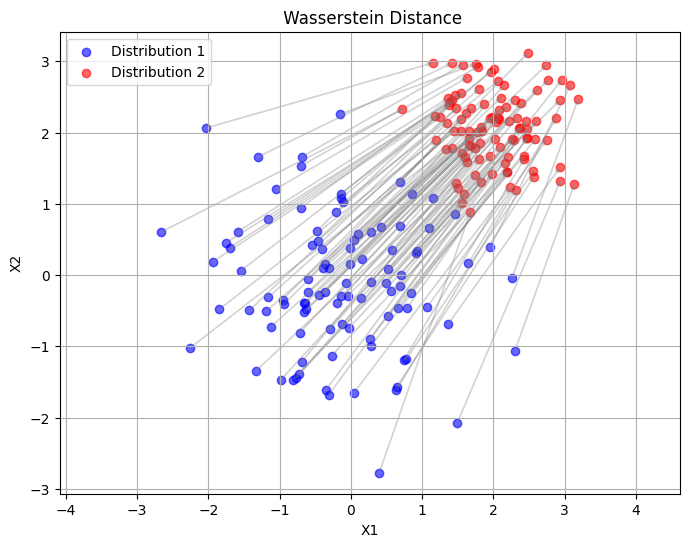
\includegraphics[width=0.5\linewidth]{3Theory/pictures/WassersteinIllustrated.png}
    \caption{Illustration of the Wasserstein distance between two distributions. The distance is the average distance between the points in the two distributions.}
    \label{fig:WassersteinDistance}
\end{figure}


In one dimension the Wasswerstein distance can be written as 
\begin{align*}
    W_p(\mu,\nu) = \int_{0}^1 |F_\mu(q)^{-1} - F_\nu(q)^{-1}|^p dq.
\end{align*}
From this we obtain through a change of variables that the Wasserstein distance can be written as
\begin{align*}
    W_p(\mu,\nu) = \left( \int_{\mathbb{R}} |F_\mu(x) - F_\nu(x)|^p dx \right)^{\frac{1}{p}}. 
\end{align*}

This motivates how the difference between two \gls{CDF}s can be used as a distance measure. Note that the following can no longer be called the Wasserstein distance. In two dimensions we therefore define a distance measure between distributions as
\begin{align*}
    d(\mu,\nu) = \left(\iint_{\mathbb{R}^2} |F_\mu(x,y) - F_\nu(x,y)|^p dx dy \right) ^{\frac{1}{p}}.
\end{align*}
$F_\mu$ and $F_\nu$ are the \gls{CDF}s of the two distributions. These distributions are estimated using a kernel density estimation with the gaussian kernel \todo{Reference, can't find good} over a grid of points. After normalizing the densities to create a distribution, this gives estimates of the \gls{PDF}s for each data set. If computing the cumulative sum of the approximate \gls{PDF}s in each dimension we get an approximated \gls{CDF} of the data. 

The distance is then approximated by numerical integration over the grid of points as
\begin{align*}
    d(\mu,\nu) = \left( \sum_{i=1}^n \sum_{j=1}^m |\hat F_\mu(x_i,y_j) - \hat F_\nu(x_i,y_j)|^p \Delta x_i \Delta y_j \right)^{\frac{1}{p}},
\end{align*}
where $\Delta x_i$ and $\Delta y_j$ are the step sizes in the $x$ and $y$ dimensions respectively. The distance is then calculated as the average distance between the two distributions. The density estimates and the corresponding CDFs are illustrated in \Cref{fig:ApproxWasserstein}. The estimated \gls{PDF}s are shown in \Cref{fig:density1} and \Cref{fig:density2}. The estimated \gls{CDF}s are shown in \Cref{fig:dist1} and \Cref{fig:dist2}. The difference between the two distributions is shown in \Cref{fig:diffDist1and2} and the distance approximation is then calculated as the average distance between the two distributions. That is, the integral under the difference between the two distributions. 


\begin{figure}
    \centering
    \begin{subfigure}{0.45\textwidth}
        \centering
        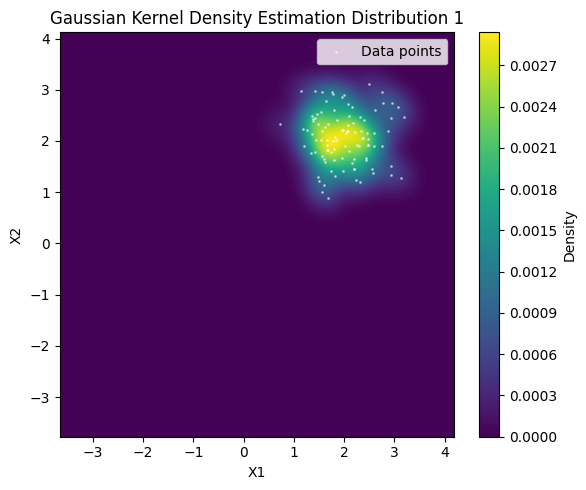
\includegraphics[width=\textwidth]{3Theory/pictures/densityDist1.png}
        \caption{}
        \label{fig:density1}
    \end{subfigure}
    \hfill
    \begin{subfigure}{0.45\textwidth}
        \centering
        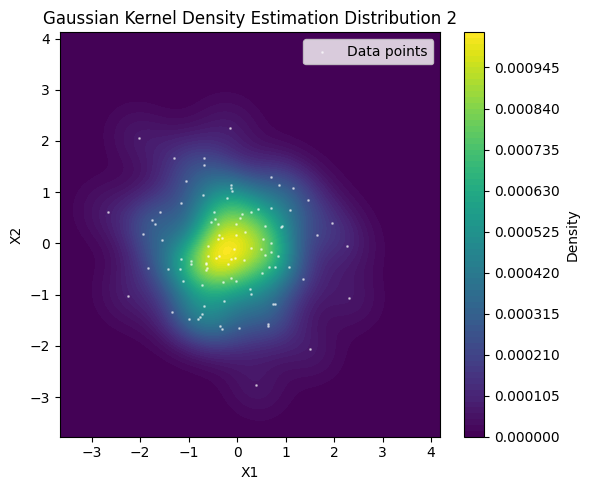
\includegraphics[width=\textwidth]{3Theory/pictures/densityDist2.png}
        \caption{}
        \label{fig:density2}
    \end{subfigure}
    \vfill
    \begin{subfigure}{0.45\textwidth}
        \centering
        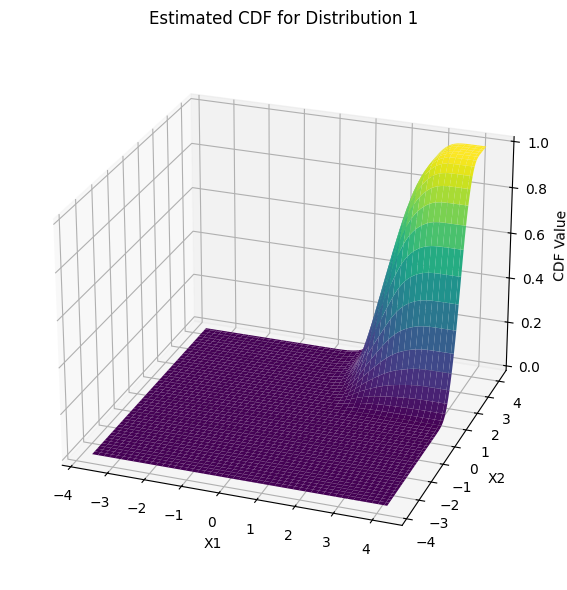
\includegraphics[width=\textwidth]{3Theory/pictures/CDFDist1.png}
        \caption{}
        \label{fig:dist1}
    \end{subfigure}
    \hfill
    \begin{subfigure}{0.45\textwidth}
        \centering
        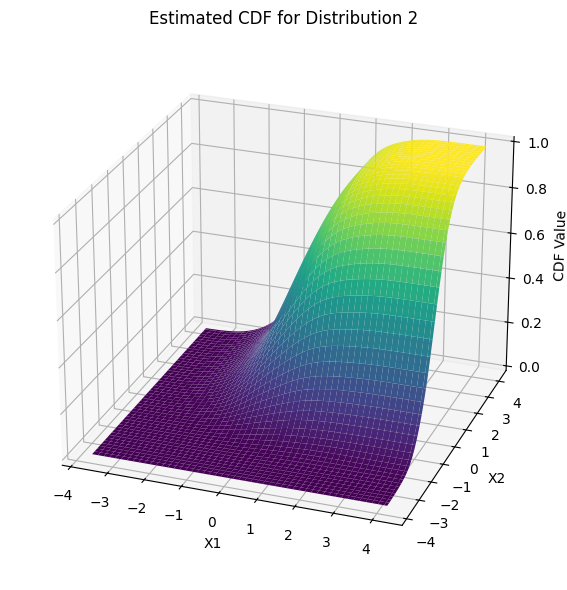
\includegraphics[width=\textwidth]{3Theory/pictures/CDFDist2.png}
        \caption{}
        \label{fig:dist2}
    \end{subfigure}
    
    \vfill
    \begin{subfigure}{0.45\textwidth}
        \centering
        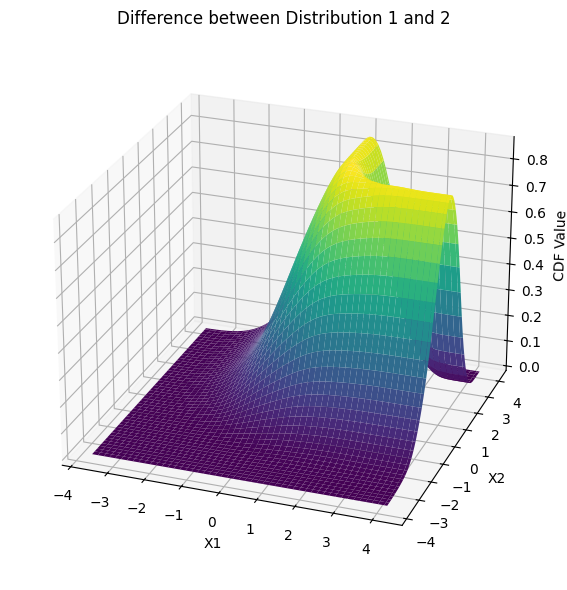
\includegraphics[width=\textwidth]{3Theory/pictures/diffDist1and2.png}
        \caption{}
        \label{fig:diffDist1and2}
    \end{subfigure}
    \caption{Density and CDF plots used in the Wasserstein distance calculation.}
    \label{fig:ApproxWasserstein}
\end{figure}

